
\section{Παραλλαγή του Logistic Χάρτη}


Μελετήθηκε η δυναμική συμπεριφορά της εξίσωσης διακριτού χρόνου:

	\begin{equation}
		x_i=k*(a+x_{i-1})^2 *(b-x_{i-1}))
		\label{f:x1}
	\end{equation}


	όπου a,b,k, q:παράμετροι\\\\
	
	Για την εύρεση της δυναμικής συμπεριφοράς του συστήματος εξετάστηκε μια περιοχή τιμών των συγκεκριμένων παραμέτρων, ώστε να επιτευχθεί ταυτόχρονη σύγκριση της περιοδικής και χαοτικής συμπεριφοράς του. Πιο συγκεκριμένα, στη μελέτη που πραγματοποιήθηκε οι παράμετροι a, b, κρατήθηκαν αρχικά σταθερές με τιμές a=1, b=2  όπως και η αρχική συνθήκη του x1 =0.1 παρέμεινε  σταθερή,  ενώ η τιμή της παραμέτρου q μεταβάλλονταν στο διάστημα[0.1,1.7] με βήμα 0.2. Έτσι, για κάθε περίπτωση παράχθηκαν το διάγραμμα διακλάδωσης, ο εκθέτης Lyapunov και το διάγραμμά της τιμής xi σε συνάρτηση με την τιμή xi-1., τα οποία παρουσιάζονται και αναλύονται στη συνέχεια.
	
\subsection{Για q=-0.1}


	
Στο σχήμα \ref{f:g1} παρατίθεται το διάγραμμα διακλάδωσης του συστήματος \ref{f:x1}, ως προς την παράμετρο k, για a=1, b=2 και q =- 0.1. Για αυτές τις τιμές των παραμέτρων το σύστημα ξεκινάει από περίοδο-1 για k = 0.3 , ενώ για  k = 0.4 εμφανίζει τον πρώτο διπλασιασμό της περιόδου. Τον δεύτερο διπλασιασμό τον εμφανίζει για k=0.47 (περίοδος-4) ,τον τρίτο για k=0.476(περίοδος-8) . Ενώ ο τελευταίος διπλασιασμός εμφανίζεται λίγο πιο μετά τον τρίτο για k=0.478 (περίοδος-16). Στην συνέχεια για k>0.479το σύστημα εισέρχεται στο χάος , μέχρι να εξέλθει  για k=0.51(περίοδος-3) και να ξανά εισέλθει σε χάος μετά από δύο διπλασιασμούς k=0.52(περίοδος-6) και k=0.522(περίοδος-11) για k>0.524. To φαινόμενο αυτό είναι γνωστό ως συνοριακή κρίση .Εξέρχεται για τελευταία φορά από το χάος για k=0.555 (περίοδος-4). Για k=0.559 εμφανίζεται ένας διπλασιασμός (περίοδος-8) ο οποίος καταστρέφεται για k=0.567 , οπότε εδώ παρατηρούμε αντιμονοτονικότητα δηλαδή έχουμε μία ανάστροφη ακολουθία διπλασιασμού της περιόδου για k=0.568. Λόγω αυτού του φαινομένου το οποίο συνεχίζει μέχρι το q=-0.2,μελετήθηκε περαιτέρω το σύστημα από -0.1<q<-0.2.Τέλος για k=0.5735 έχουμε έναν τελευταίο διπλασιασμό(περίοδος-6) πριν ξανά εισέλθει το σύστημα για k>0.575 στο χάος.
Στο σχήμα \ref{f:g2} παρατίθενται 3 διαγράμματα διακλάδωσης \ref{f:g3}, \ref{f:g4}, \ref{f:g5}, \ref{f:g6}
για 0.54<k<0.6. Ουσιαστικά εστιάστηκε το διάγραμμα στην αντιμονοτονικότητα που εμφανίζεται για τις συγκεκριμένες τιμές του q. Επίσης παρατηρούμε στα διαγράμματα \ref{f:g4}, \ref{f:g5}, \ref{f:g6} δημιουργία χαοτικών φυσαλίδων. Δηλαδή, το σύστημα εισέρχεται στο χάος με διπλασιασιασμό της περιόδου και στην συνέχεια εξέρχεται από αυτό με αντίστροφο διπλασιασμό της περιόδου. Επιπλέον στο διάγραμμα \ref{f:g6} το φαινόμενο εμφανίζεται δυο φορές  για 0.560<k<0.568 και 0.571<k<0.573. 
Επιπλέον, στο σχήμα \ref{f:g7} παρατίθεται το διάγραμμα των εκθετών Lyapunov για τιμές του k στο ίδιο διάστημα τιμών [0.3, 0.6].  Στο διάστημα τιμών   k=0.522 , στο 0.51<k<0.522, και στο 0.554<k<0.574 παρατηρούμε ότι ο εκθέτης Lyapunov είναι συνεχώς αρνητικός, γεγονός που επιβεβαιώνει την περιοδική συμπεριφορά του συστήματος. Ενώ στα υπόλοιπα διαστήματα ο θετικός εκθέτης Lyapunov υποστηρίζει την χαοτική του συμπεριφορά, όπως έγινε φανερό και από το διάγραμμα διακλάδωσης.
Τέλος, στον Πίνακα \ref{tab:abc} παρατίθενται ενδεικτικές τιμές της παραμέτρου k και η συμπεριφορά που παρουσιάζει το σύστημα για αυτές, σύμφωνα με το διάγραμμα διακλάδωσης, καθώς και τα αντίστοιχα σχήματα των διαγραμμάτων της τιμής \(x_i\) σε συνάρτηση με την τιμή \(x_{i+1}\). Από τα παραγόμενα σχήματα προκύπτει αριθμός σημείων αντίστοιχος με την περίοδο του συστήματος.


\begin{table}[h!]
	\centering
	\begin{tabular}{l | l | l}
		Παράμετρος k & Συμπεριφορά & Σχήμα\\
		\hline
		0.3 &  Περίοδος-1 & \ref{f:k1}\\
		0.41 & Περίοδος-2 & \ref{f:k2}\\
		0.476 &  Περίοδος-8 & \ref{f:k3}\\
		0.4778 & Περίοδος-16 & \ref{f:k4}\\
		0.479 & Χάος & \ref{f:k5}\\
		0.517 & Περίοδος-3 & \ref{f:k6})\\
		0.52 & Περίοδος-6 & \ref{f:k7}\\
		0.522 & Περίοδος-11 & \ref{f:k8}\\
		0.524 & Χάος & \ref{f:k9}\\
		0.555 & Περίοδος-4 & \ref{f:k10}\\
		0.559 & Περίοδος-8 & \ref{f:k11}\\
		0.568 & Περίοδος-4 & \ref{f:k12}\\
		0.5735 & Περίοδος-6 & \ref{f:k13}\\
		0.575 & Χάος & \ref{f:k14}\\
	\end{tabular}
	\caption{ Συμπεριφορά του υπό μελέτη συστήματος για διάφορες τιμές του k,για a=1, b=2 και q=-0.1}
	\label{tab:abc}
\end{table}


\begin{figure}[h!]
	\centering
	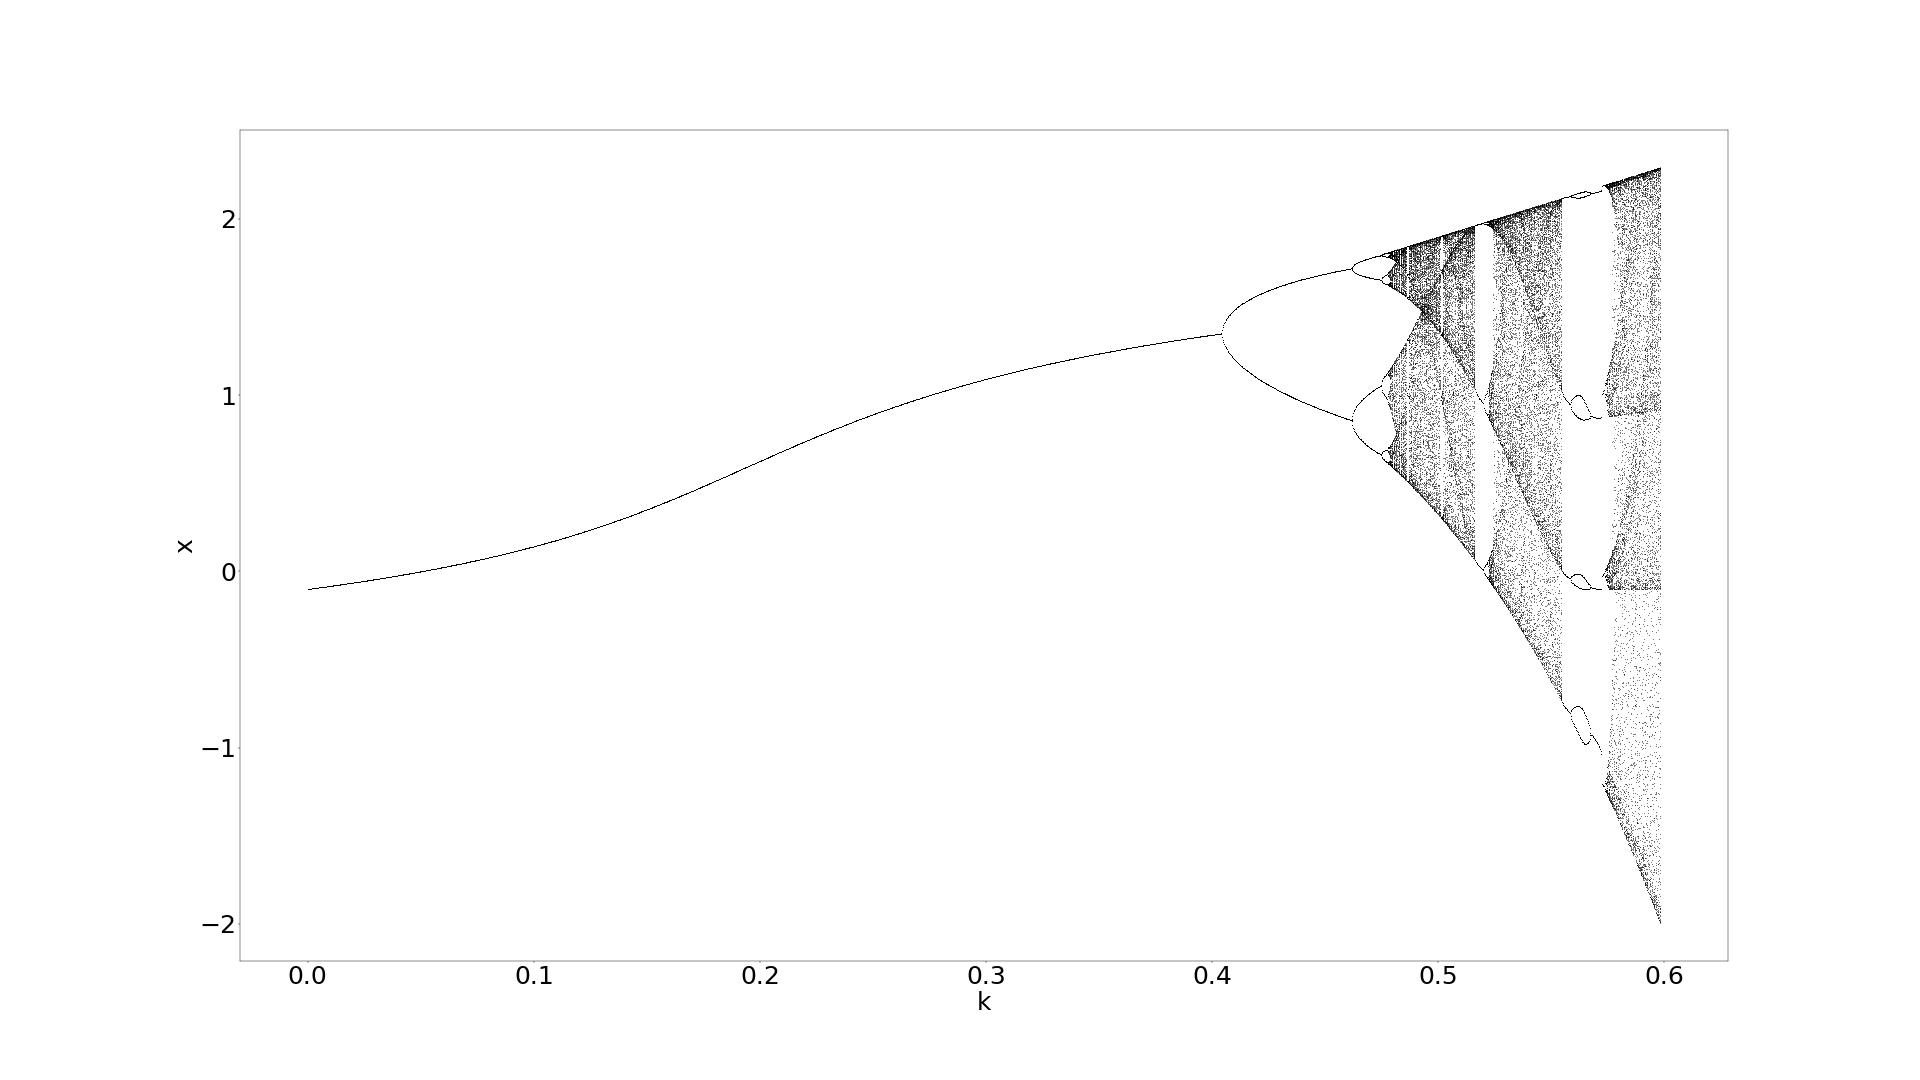
\includegraphics[width=0.8\linewidth]{LateX images/graphs/g1}
	\caption{ Διάγραμμα διακλάδωσης, για a=1, b=2 και q=-0.1}
	\label{f:g1}
\end{figure}



\begin{figure}[h!]
	\centering

	\begin{subfigure}[b]{0.4\textwidth}
		\centering
		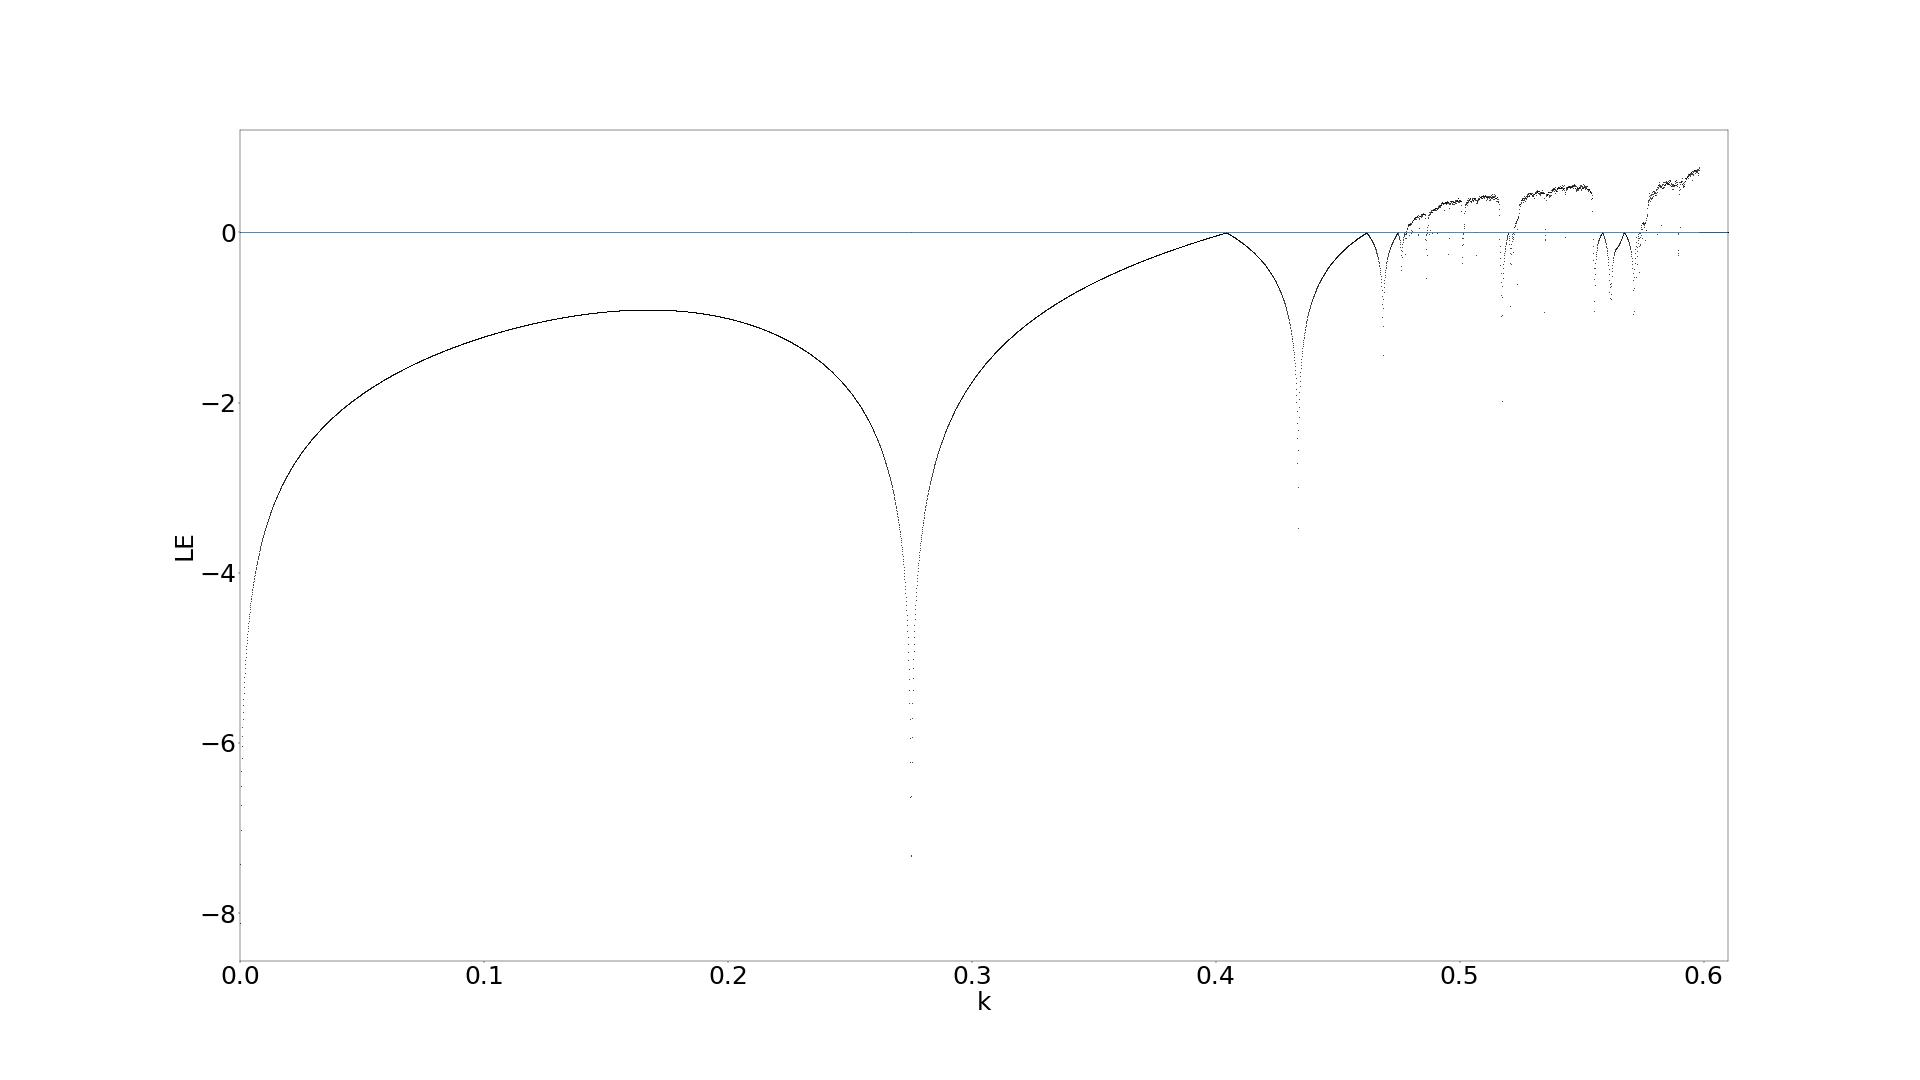
\includegraphics[width=\textwidth]{LateX images/graphs/g2}
		\caption{q=-0.112}
		\label{f:g3}
	\end{subfigure}
	\hfill
	\begin{subfigure}[b]{0.4\textwidth}
		\centering
		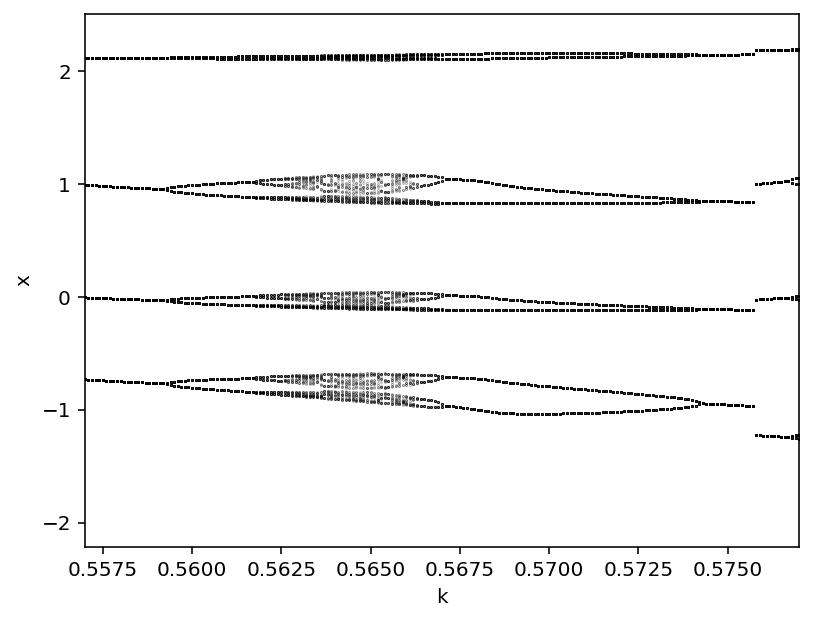
\includegraphics[width=\textwidth]{LateX images/graphs/g3}
		\caption{q=-0.114}
		\label{f:g4}
	\end{subfigure}
	\hfill
	\begin{subfigure}[b]{0.4\textwidth}
		\centering
		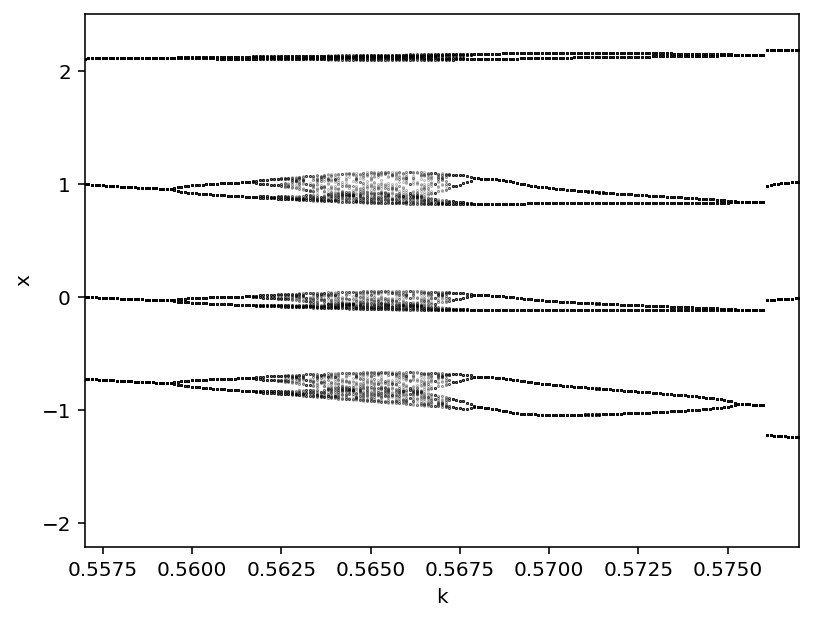
\includegraphics[width=\textwidth]{LateX images/graphs/g4}
		\caption{q=-0.116}
		\label{f:g5}
	\end{subfigure}
	\hfill
	\begin{subfigure}[b]{0.4\textwidth}
		\centering
		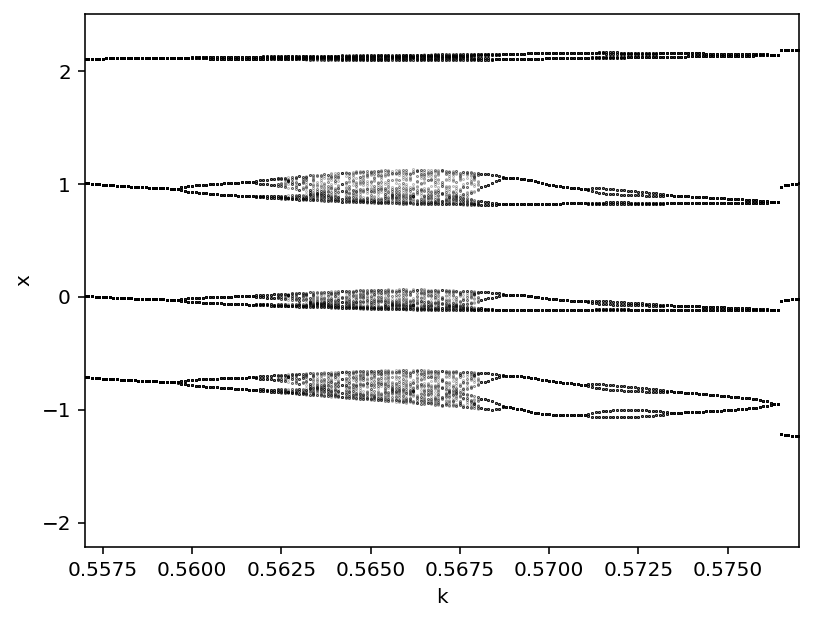
\includegraphics[width=\textwidth]{LateX images/graphs/g5}
		\caption{q=-0.118}
		\label{f:g6}
	\end{subfigure}
\caption{Διάγραμμα διακλάδωσης, για :}
\label{f:g2}
\end{figure}

\begin{figure}[h!]
	\centering
	\includegraphics[width=0.6\linewidth]{"LateX images/graphs/g6 "}
	\caption{Διάγραμμα του εκθέτη Lyapunov σε συνάρτηση με την παράμετρο k, για a=1, b=2 και q=-0.1.}
	\label{f:g7}
\end{figure}


\begin{figure}[h!]
	\centering	
	\begin{subfigure}[b]{0.4\linewidth}
		\centering
		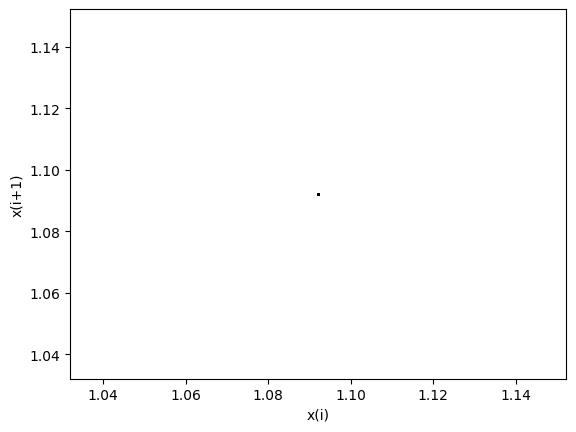
\includegraphics[width=\linewidth]{LateX images/graphs/k03}
		\caption{Για k=0.3}
		\label{f:k1}
	\end{subfigure}
	\hfill
	\begin{subfigure}[b]{0.4\textwidth}
		\centering
		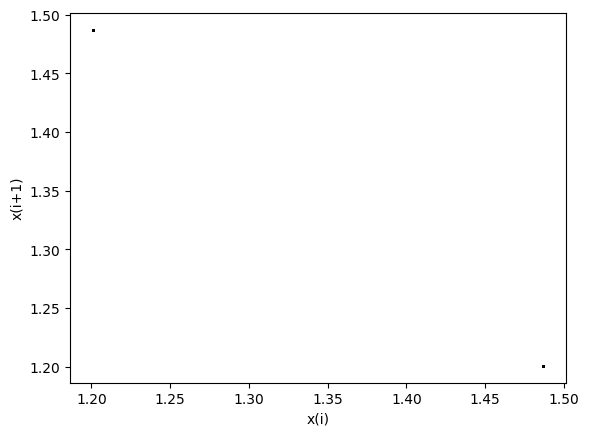
\includegraphics[width=\textwidth]{LateX images/graphs/k041}
		\caption{Για k=0.41}
		\label{f:k2}
	\end{subfigure}
	\hfill
	\begin{subfigure}[b]{0.4\textwidth}
		\centering
		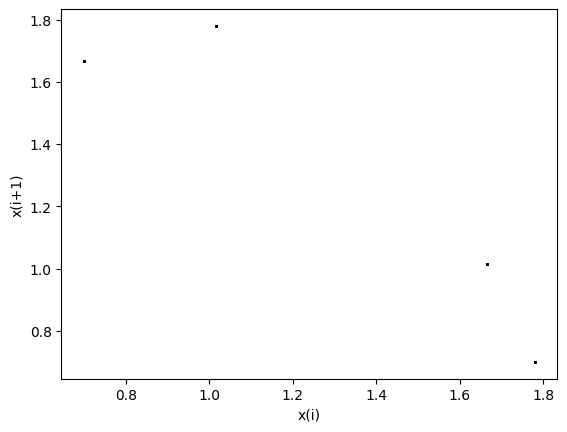
\includegraphics[width=\textwidth]{LateX images/graphs/k047}
		\caption{Για k=0.047}
		\label{f:k3}
	\end{subfigure}
	\hfill
	\begin{subfigure}[b]{0.4\textwidth}
		\centering
		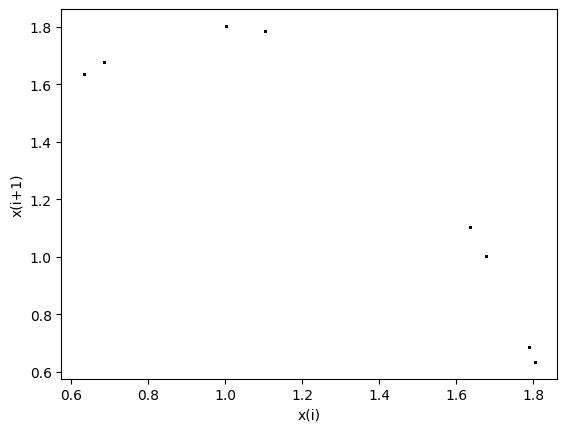
\includegraphics[width=\textwidth]{LateX images/graphs/k0476}
		\caption{Για k=0.476}
		\label{f:k4}
	\end{subfigure}
	\hfill
	\begin{subfigure}[b]{0.4\textwidth}
		\centering
		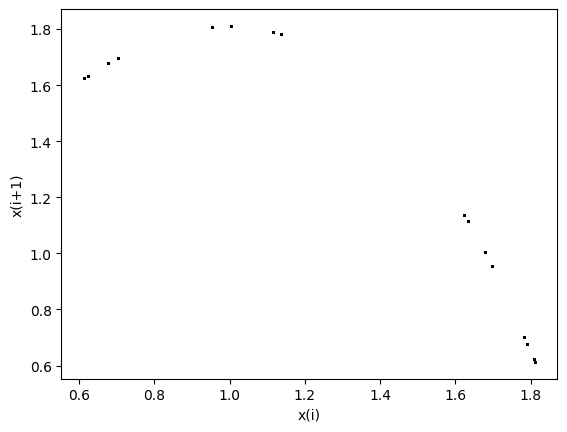
\includegraphics[width=\textwidth]{LateX images/graphs/k04778}
		\caption{Για k=0.4778}
		\label{f:k5}
	\end{subfigure}
	\hfill
	\begin{subfigure}[b]{0.4\textwidth}
		\centering
		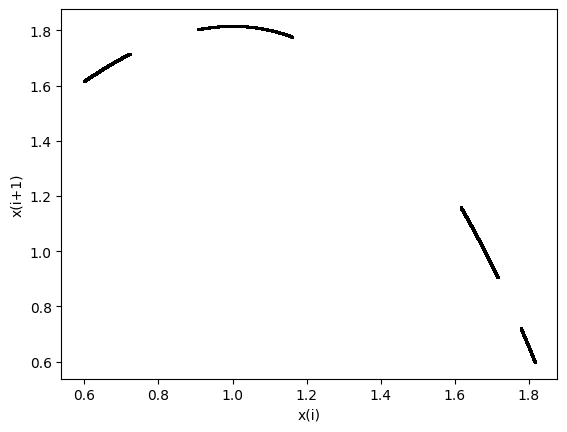
\includegraphics[width=\textwidth]{LateX images/graphs/k0479}
		\caption{Για k=0.479}
		\label{f:k6}
	\end{subfigure}
	\hfill	
	\begin{subfigure}[b]{0.4\textwidth}
		\centering
		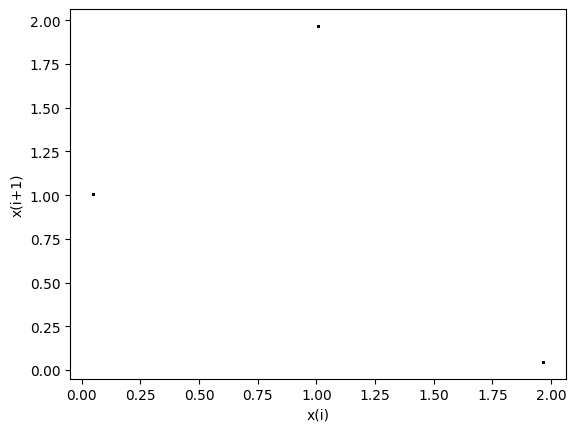
\includegraphics[width=\textwidth]{LateX images/graphs/k0517}
		\caption{Για k=0.517}
	\end{subfigure}
	\hfill
	\begin{subfigure}[b]{0.4\textwidth}
		\centering
		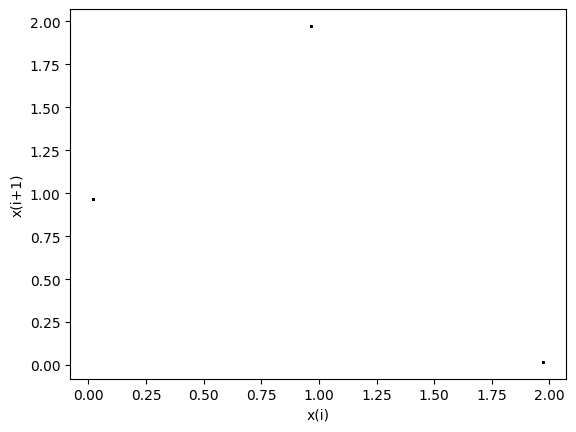
\includegraphics[width=\textwidth]{LateX images/graphs/k0519}
		\caption{Για k=0.519}
		\label{f:k7}
	\end{subfigure}
	\hfill
\caption{Διαγράμματα της τιμής \(x_i\) με την τιμή \(x_{i+1}\) α'μέρος:}
\end{figure}

\begin{figure}[h!]
	\centering
	\begin{subfigure}[c]{0.4\textwidth}
		\centering
		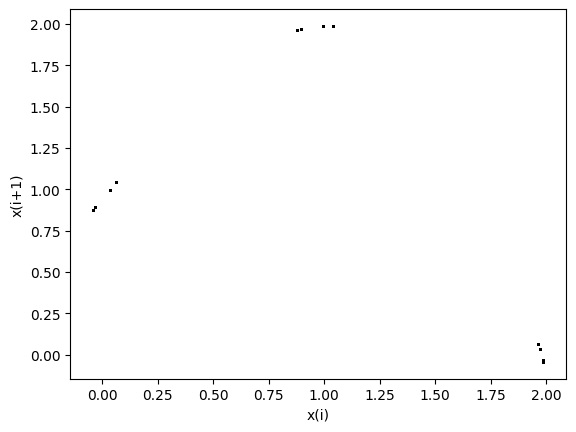
\includegraphics[width=\textwidth]{LateX images/graphs/k0522}
		\caption{Για k=0.522}
		\label{f:k8}
	\end{subfigure}
	\hfill
	\begin{subfigure}[c]{0.4\textwidth}
		\centering
		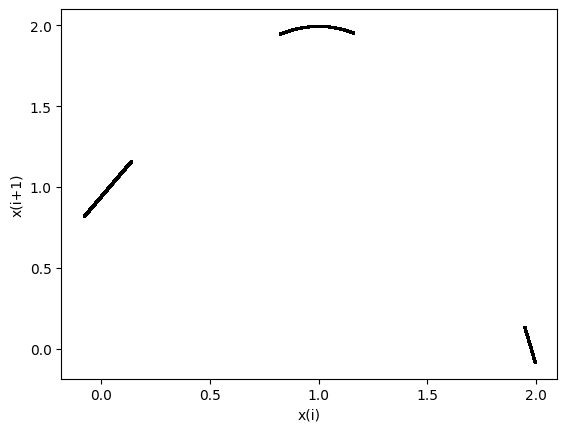
\includegraphics[width=\textwidth]{LateX images/graphs/k0524}
		\caption{Για k=0.524}
		\label{f:k9}
	\end{subfigure}
	\hfill
	\begin{subfigure}[c]{0.4\textwidth}
		\centering
		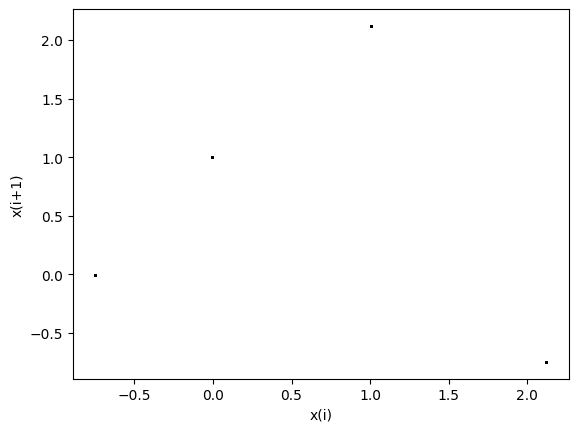
\includegraphics[width=\textwidth]{LateX images/graphs/k0555}
		\caption{Για k=0.555}
		\label{f:k10}
	\end{subfigure}
	\hfill
	\begin{subfigure}[c]{0.4\textwidth}
		\centering
		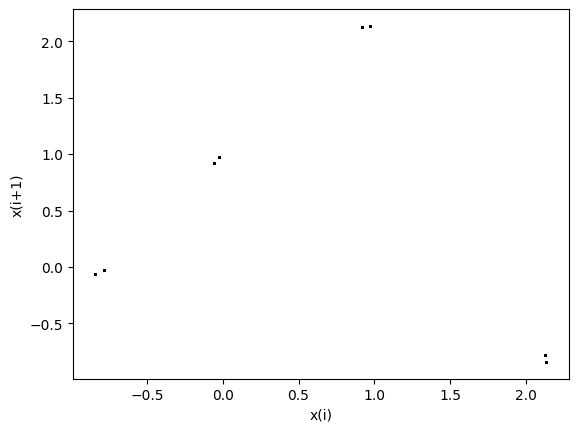
\includegraphics[width=\textwidth]{LateX images/graphs/k0559}
		\caption{Για k=0.559}
		\label{f:k11}
	\end{subfigure}
	\hfill
	\begin{subfigure}[c]{0.4\textwidth}
		\centering
		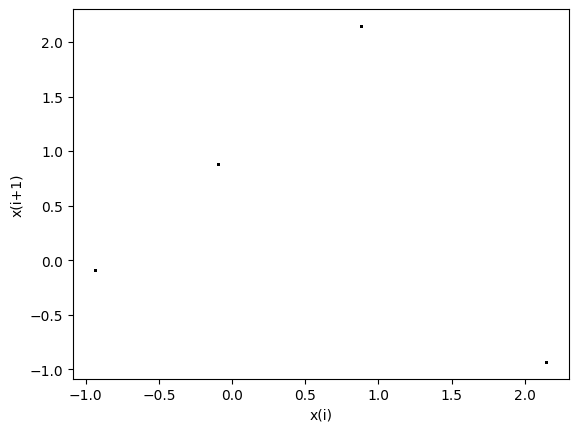
\includegraphics[width=\textwidth]{LateX images/graphs/k0568}
		\caption{Για k=0.568}
		\label{f:k12}
	\end{subfigure}
	\hfill
	\begin{subfigure}[c]{0.4\textwidth}
		\centering
		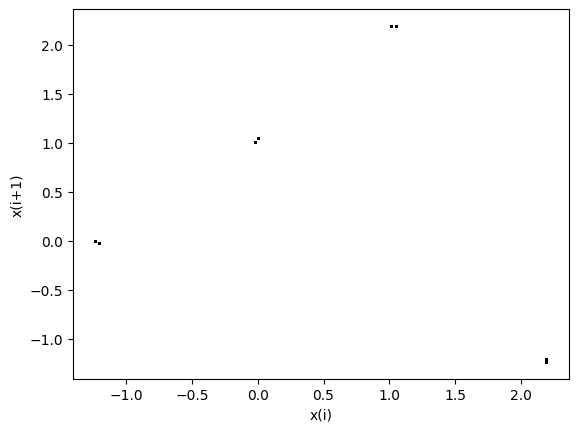
\includegraphics[width=\textwidth]{LateX images/graphs/k05735}
		\caption{Για k=0.5735}
		\label{f:k13}
	\end{subfigure}
	\hfill
	\begin{subfigure}[c]{0.4\textwidth}
		\centering
		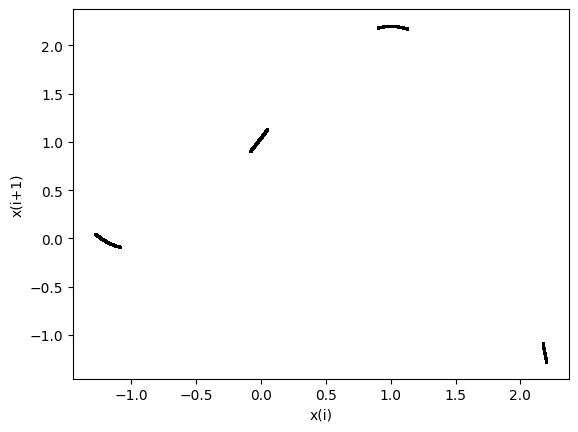
\includegraphics[width=\textwidth]{LateX images/graphs/k0575}
		\caption{Για k=0.575}
		\label{f:k14}
	\end{subfigure}
\caption{Διαγράμματα της τιμής \(x_i\) με την τιμή \(x_{i+1}\) β'μέρος:}
\end{figure}
\vfill
\clearpage
\newpage
\subsection{Για q=-0.3}

Στο σχήμα \ref{f:g8} παρατίθεται το διάγραμμα διακλάδωσης του συστήματος \ref{f:x1}, ως προς την παράμετρο k, για a=1, b=2 και q =- 0.3. Για αυτές τις τιμές των παραμέτρων το σύστημα ξεκινάει από περίοδο-1 για k = 0.3 , ενώ για  k = 0.44 εμφανίζει τον πρώτο διπλασιασμό της περιόδου. Τον δεύτερο διπλασιασμό τον εμφανίζει για k=0.5 (περίοδος-4) ,τον τρίτο για k=0.511(περίοδος-8).Στην συνέχεια για k>0.5165 το σύστημα εισέρχεται στο χάος , μέχρι να εξέλθει  για k=0.551(περίοδος-3) και να ξανά εισέλθει σε χάος μετά από δύο διπλασιασμούς k=0.555(περίοδος-6) και k=0.556(περίοδος-12) για k>0.5573. To φαινόμενο αυτό είναι γνωστό ως συνοριακή κρίση .Εξέρχεται για τελευταία φορά από το χάος για k=0.583 (περίοδος-4) και μετά απο ένα διπλασιασμό  για k=0.5846(Περίόδος-7) είσέρχεται για τελευταία φορά στο χάος για k=0.5851.
Επομένως και σε αυτή την περίπτωση το σύστημα εισέρχεται στο χάος με διπλασιασμό της περιόδου. 
Επιπλέον, στο σχήμα \ref{f:g9} παρατίθεται το διάγραμμα των εκθετών Lyapunov για τιμές του k στο ίδιο διάστημα τιμών [0, 0.636].  Στο διάστημα τιμών   0<k<0.511 , στο 0.551<k<0.556, και στο 0.583<k<0.5846 παρατηρούμε ότι ο εκθέτης Lyapunov είναι συνεχώς αρνητικός, γεγονός που επιβεβαιώνει την περιοδική συμπεριφορά του συστήματος. Ενώ στα υπόλοιπα διαστήματα ο θετικός εκθέτης Lyapunov υποστηρίζει την χαοτική του συμπεριφορά, όπως έγινε φανερό και από το διάγραμμα διακλάδωσης.
Τέλος, στον Πίνακα \ref{tab:abc1} παρατίθενται ενδεικτικές τιμές της παραμέτρου k και η συμπεριφορά που παρουσιάζει το σύστημα για αυτές, σύμφωνα με το διάγραμμα διακλάδωσης, καθώς και τα αντίστοιχα σχήματα των διαγραμμάτων της τιμής \(x_i\) σε συνάρτηση με την τιμή \(x_{i+1}\). Από τα παραγόμενα σχήματα προκύπτει αριθμός σημείων αντίστοιχος με την περίοδο του συστήματος.
\begin{table}[h!]
	\centering
	\begin{tabular}{l | l | l}
		Παράμετρος k & Συμπεριφορά & Σχήμα\\
		\hline
		0.3 &  Περίοδος-1 & \ref{f:k1}\\
		0.44& Περίοδος-2 & \ref{f:k2}\\
		0.5& Περίοδος-4 & \ref{f:k2}\\
		0.511 &  Περίοδος-8 & \ref{f:k3}\\
		0.5165 & Χάος & \ref{f:k5}\\
		0.551 & Περίοδος-3 & \ref{f:k6})\\
		0.555 & Περίοδος-6 & \ref{f:k7}\\
		0.556 & Περίοδος-12 & \ref{f:k8}\\
		0.5573 & Χάος & \ref{f:k9}\\
		0.583& Περίοδος-4 & \ref{f:k10}\\
		0.5846 & Περίοδος-7 & \ref{f:k11}\\
		0.5851 & Χάος & \ref{f:k14}\\
	\end{tabular}
	\caption{ Συμπεριφορά του υπό μελέτη συστήματος για διάφορες τιμές του k,για a=1, b=2 και q=-0.3}
	\label{tab:abc1}
\end{table}

\begin{figure}[h!]
	\centering
	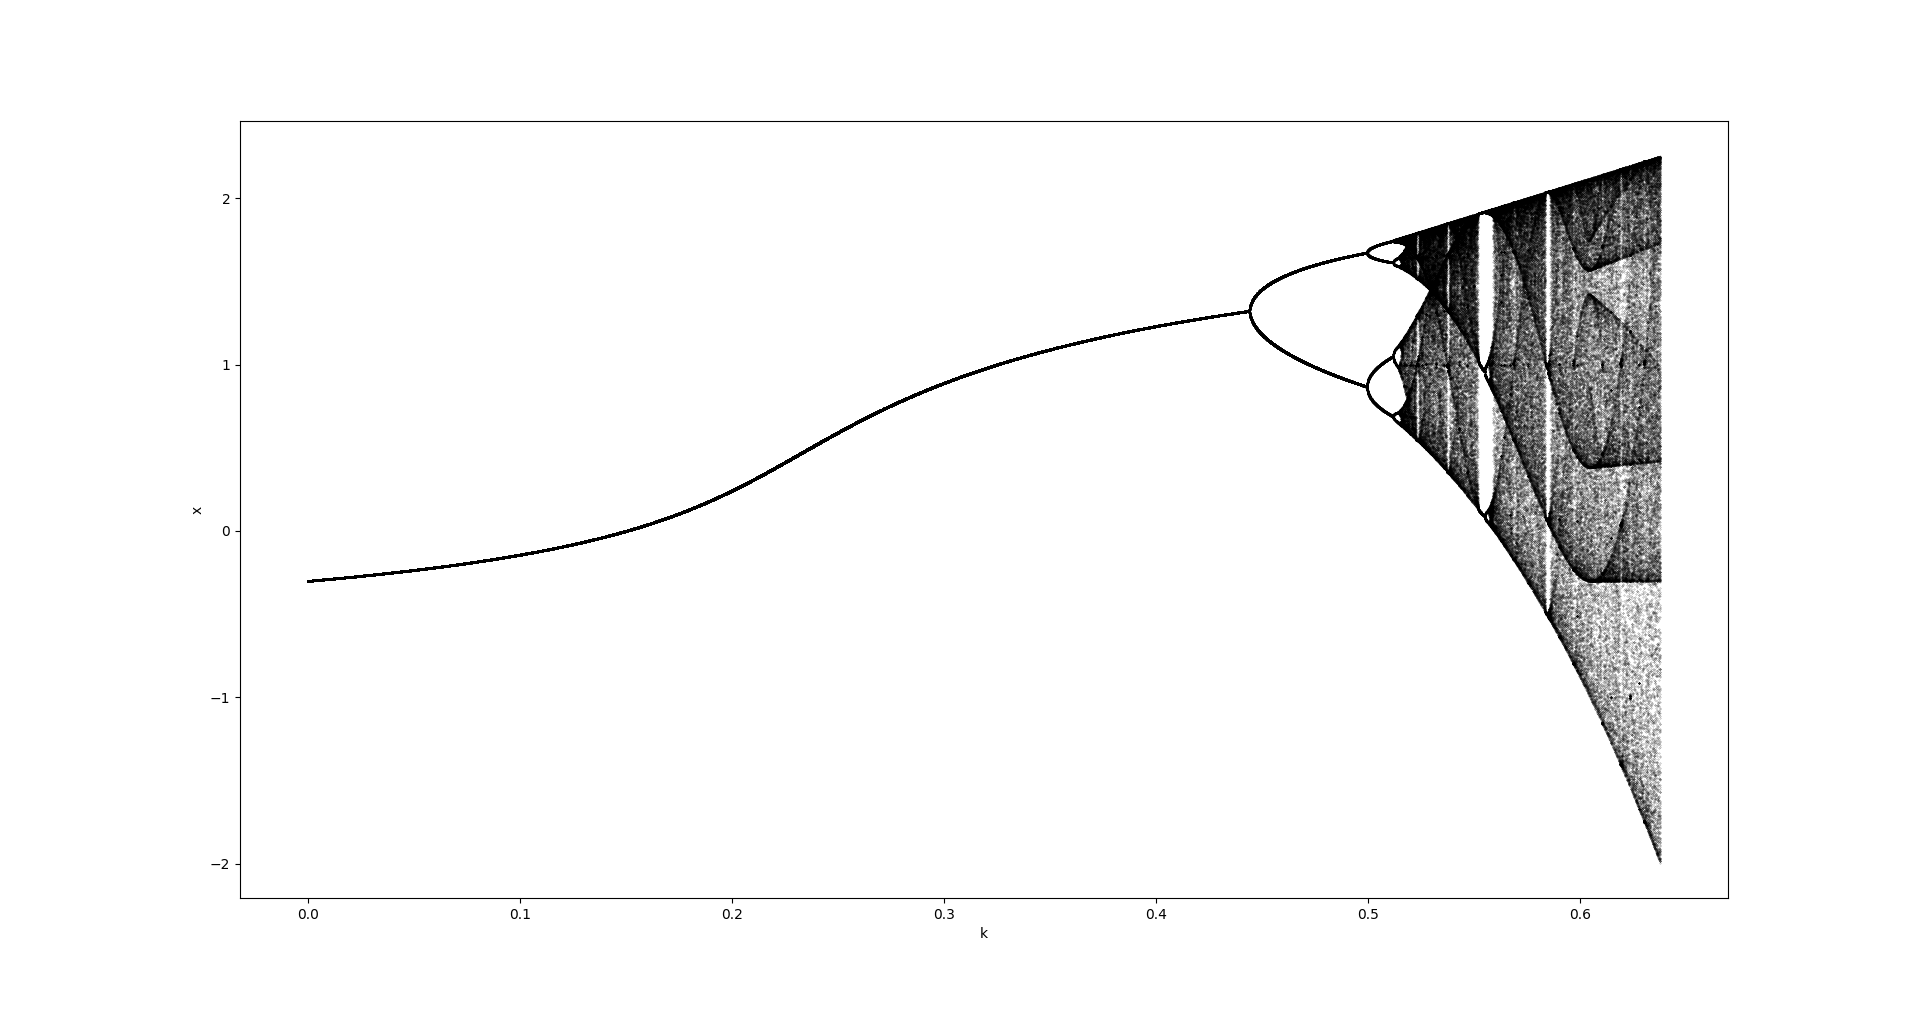
\includegraphics[width=0.8\linewidth]{LateX images/graphs q03/g1}
	\caption{ Διάγραμμα διακλάδωσης, για a=1, b=2 και q=-0.3}
	\label{f:g8}
\end{figure}

\begin{figure}[h!]
	\centering
	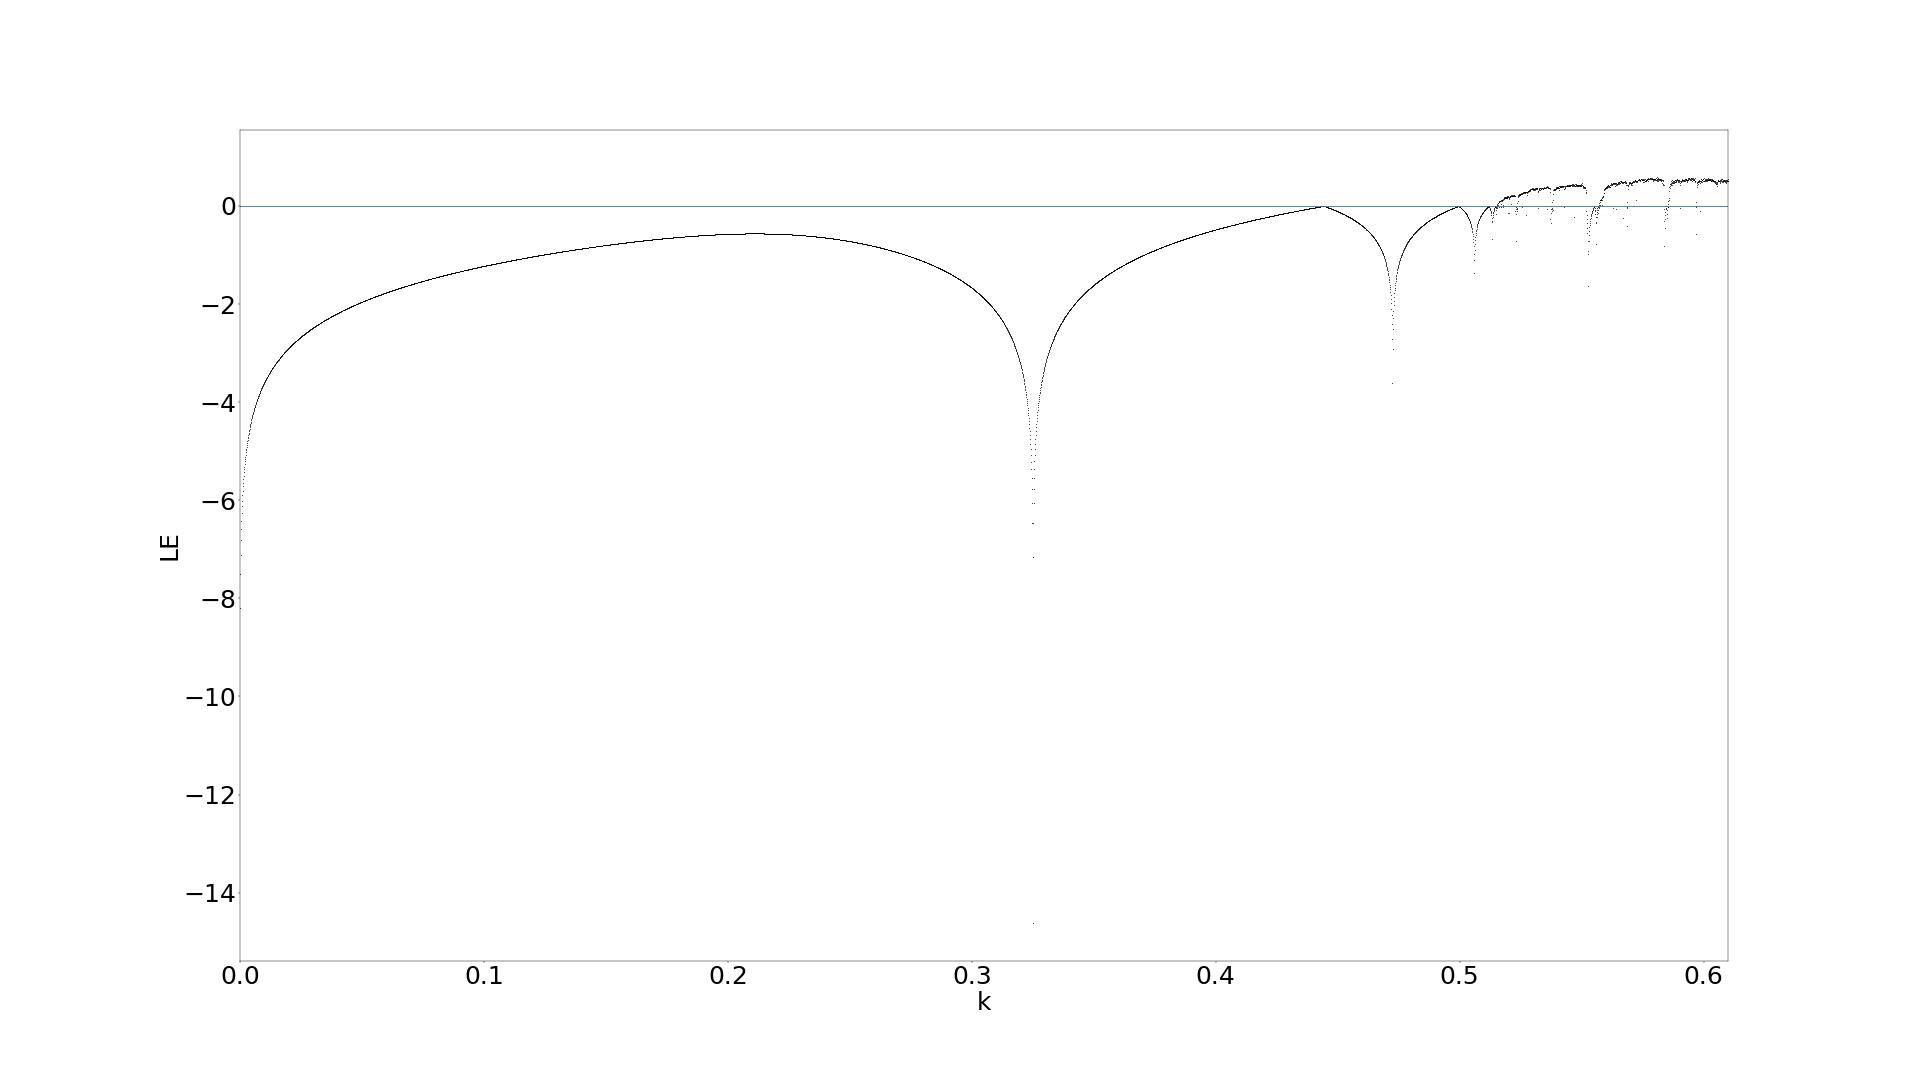
\includegraphics[width=0.6\linewidth]{LateX images/graphs q03/g2}
	\caption{ Διάγραμμα του εκθέτη Lyapunov σε συνάρτηση με την παράμετρο k, για a=1, b=2 και q=-0.3}
	\label{f:g9}
\end{figure}

\begin{figure}[h!]
	\centering	
	\begin{subfigure}[b]{0.4\textwidth}
		\centering
		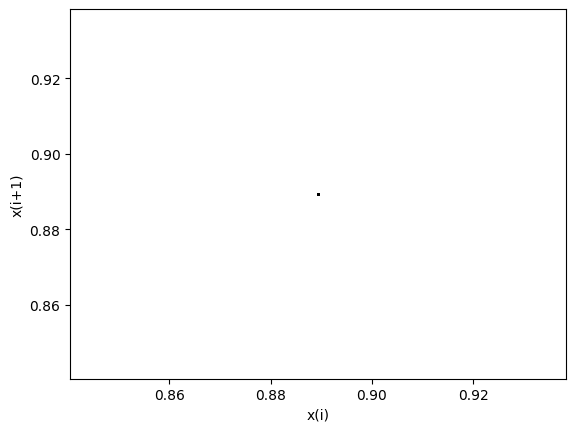
\includegraphics[width=\textwidth]{LateX images/graphs q03/g3}
		\caption{Για k=0.3}
		\label{f:k15}
	\end{subfigure}
	\hfill
	\begin{subfigure}[b]{0.4\textwidth}
		\centering
		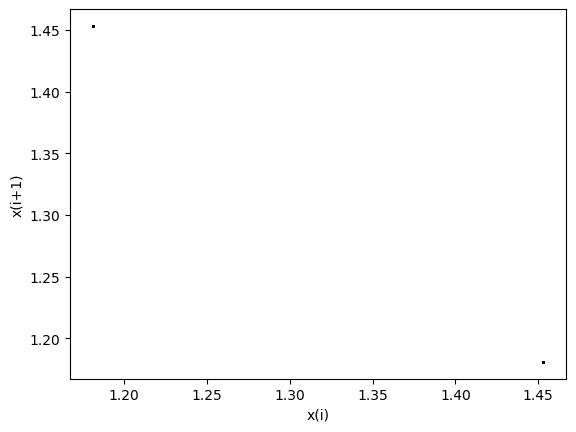
\includegraphics[width=\textwidth]{LateX images/graphs q03/g4}
		\caption{Για k=0.44}
		\label{f:k16}
	\end{subfigure}
	\hfill
	\begin{subfigure}[b]{0.4\textwidth}
		\centering
		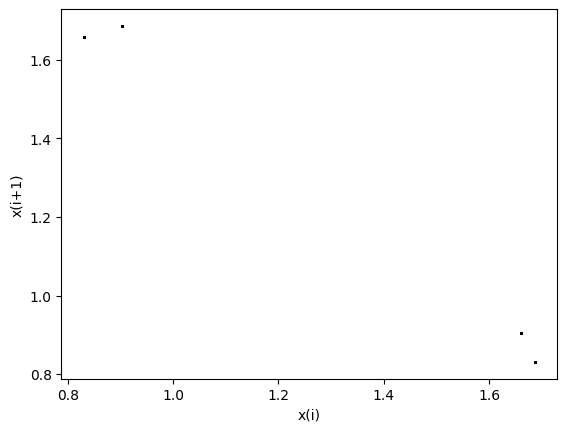
\includegraphics[width=\textwidth]{LateX images/graphs q03/g5}
		\caption{Για k=0.5}
		\label{f:k17}
	\end{subfigure}
	\hfill
	\begin{subfigure}[b]{0.4\textwidth}
		\centering
		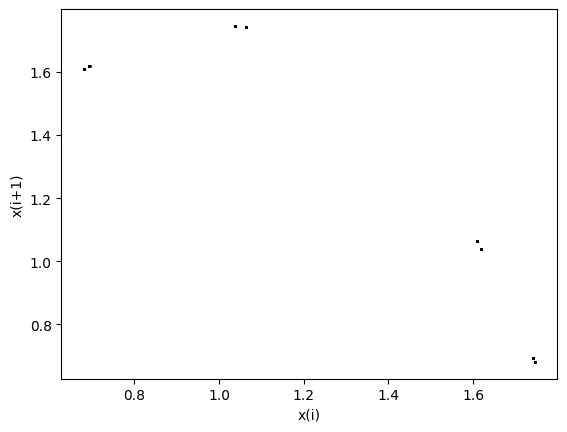
\includegraphics[width=\textwidth]{LateX images/graphs q03/g6}
		\caption{Για k=0.511}
		\label{f:k18}
	\end{subfigure}
	\hfill
	\begin{subfigure}[b]{0.4\textwidth}
		\centering
		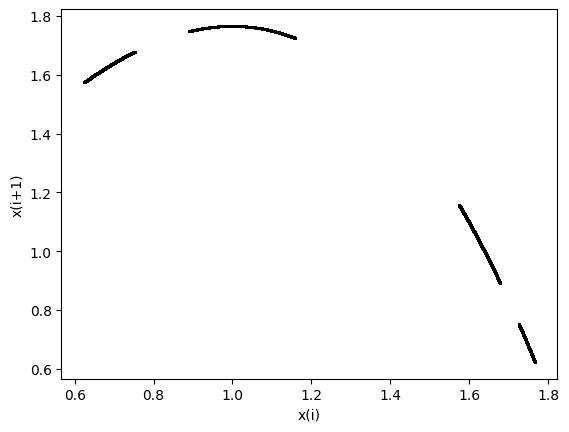
\includegraphics[width=\textwidth]{LateX images/graphs q03/g67}
		\caption{Για k=0.5165}
		\label{f:k19}
	\end{subfigure}
	\hfill
	\begin{subfigure}[b]{0.4\textwidth}
		\centering
		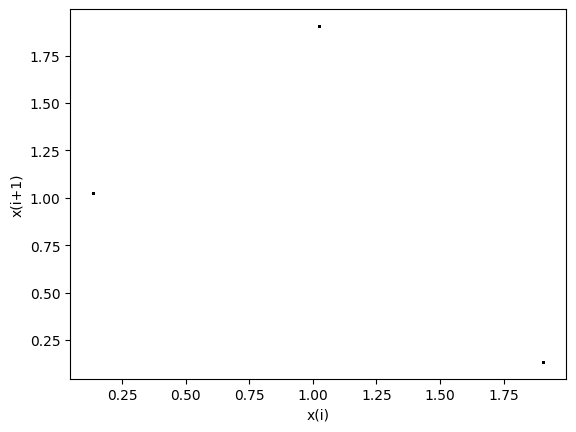
\includegraphics[width=\textwidth]{LateX images/graphs q03/g8}
		\caption{Για k=0.551}
		\label{f:k20}
	\end{subfigure}
	\hfill
\caption{Διαγράμματα της τιμής \(x_i\) με την τιμή \(x_{i+1}\) α´μέρος :}	
\end{figure}
\begin{figure}[h!]
	\centering
	
	\begin{subfigure}[b]{0.4\textwidth}
		\centering
		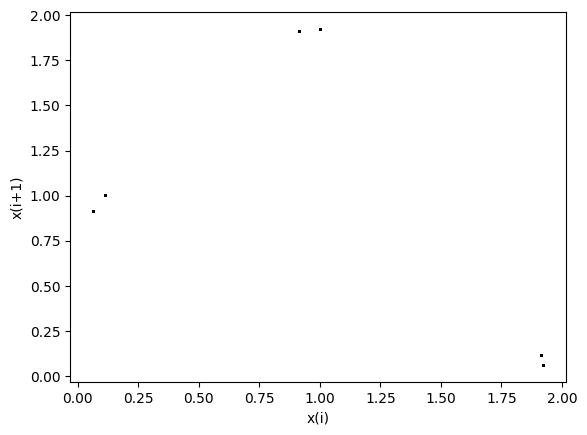
\includegraphics[width=\textwidth]{LateX images/graphs q03/g9}
		\caption{Για k=0.555}
		\label{f:k21}
	\end{subfigure}
	\hfill
	\begin{subfigure}[b]{0.4\textwidth}
		\centering
		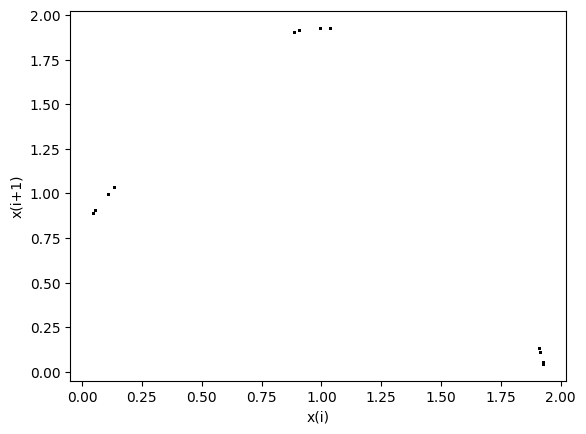
\includegraphics[width=\textwidth]{LateX images/graphs q03/g10}
		\caption{Για k=0.556}
		\label{f:k22}
	\end{subfigure}
	\hfill
	\begin{subfigure}[b]{0.4\textwidth}
		\centering
		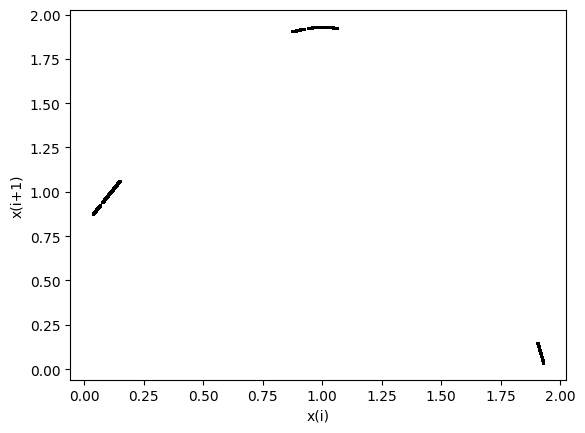
\includegraphics[width=\textwidth]{LateX images/graphs q03/g11}
		\caption{Για k=0.5573}
		\label{f:k23}
	\end{subfigure}
	\hfill
	\begin{subfigure}[b]{0.4\textwidth}
		\centering
		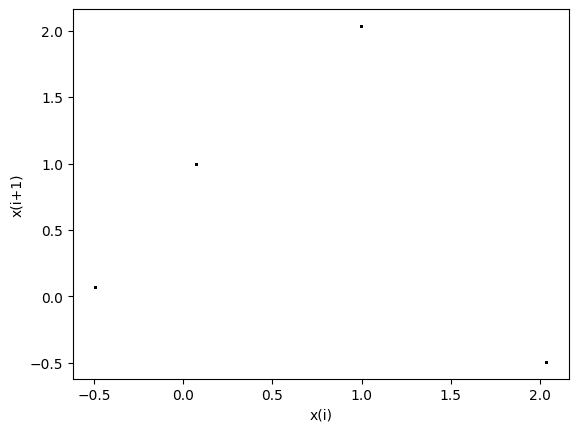
\includegraphics[width=\textwidth]{LateX images/graphs q03/g12}
		\caption{Για k=0.583}
		\label{f:k24}
	\end{subfigure}
	\hfill
	\begin{subfigure}[b]{0.4\textwidth}
		\centering
		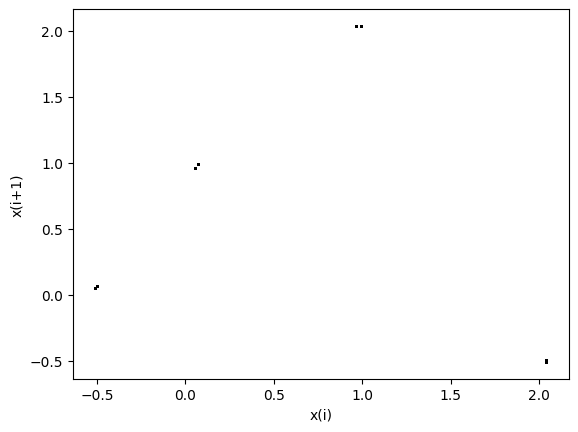
\includegraphics[width=\textwidth]{LateX images/graphs q03/g13}
		\caption{Για k=0.5846}
		\label{f:k25}
	\end{subfigure}
	\hfill
	\begin{subfigure}[b]{0.4\textwidth}
		\centering
		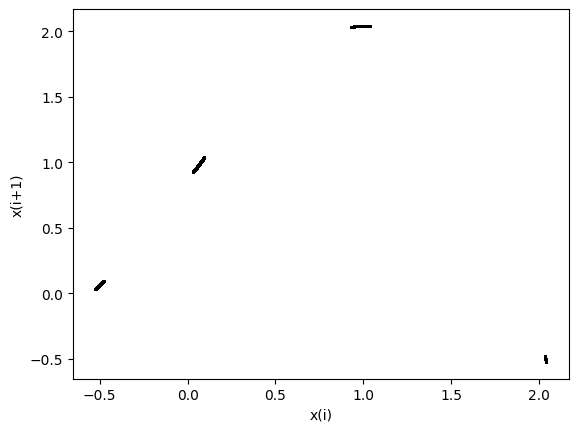
\includegraphics[width=\textwidth]{LateX images/graphs q03/g14}
		\caption{Για k=0.5851}
		\label{f:k26}
	\end{subfigure}
\caption{Διαγράμματα της τιμής \(x_i\) με την τιμή \(x_{i+1}\) β´μέρος :}	
\end{figure}

\clearpage

\subsection{Για q=-0.5}

Στο σχήμα \ref{f:g10} παρατίθεται το διάγραμμα διακλάδωσης του συστήματος \ref{f:x1}, ως προς την παράμετρο k, για a=1, b=2 και q =- 0.5. Για αυτές τις τιμές των παραμέτρων το σύστημα ξεκινάει από περίοδο-1 για k = 0.3 , ενώ για  k = 0.48 εμφανίζει τον πρώτο διπλασιασμό της περιόδου. Τον δεύτερο διπλασιασμό τον εμφανίζει για k=0.53 (περίοδος-4) ,τον τρίτο για k=0.55 (περίοδος-8) και τον τέταρτο για k=0.5531 (περόδος-15).Στην συνέχεια για k>0.5534 το σύστημα εισέρχεται στο χάος , μέχρι να εξέλθει  για k=0.59(περίοδος-3) και να ξανά εισέλθει σε χάος μετά από δύο διπλασιασμούς k=0.59377 (περίοδος-6) ,για k>0.594.
Επομένως και σε αυτή την περίπτωση το σύστημα εισέρχεται στο χάος με διπλασιασμό της περιόδου. 
Επιπλέον, στο σχήμα \ref{f:g11} παρατίθεται το διάγραμμα των εκθετών Lyapunov για τιμές του k στο ίδιο διάστημα τιμών [0, 0.679].  Στο διάστημα τιμών   0<k<0.5534 , στο 0.59<k<0.594 παρατηρούμε ότι ο εκθέτης Lyapunov είναι συνεχώς αρνητικός, γεγονός που επιβεβαιώνει την περιοδική συμπεριφορά του συστήματος. Ενώ στα υπόλοιπα διαστήματα ο θετικός εκθέτης Lyapunov υποστηρίζει την χαοτική του συμπεριφορά, όπως έγινε φανερό και από το διάγραμμα διακλάδωσης.
Τέλος, στον Πίνακα \ref{tab:abc2} παρατίθενται ενδεικτικές τιμές της παραμέτρου k και η συμπεριφορά που παρουσιάζει το σύστημα για αυτές, σύμφωνα με το διάγραμμα διακλάδωσης, καθώς και τα αντίστοιχα σχήματα των διαγραμμάτων της τιμής \(x_i\) σε συνάρτηση με την τιμή \(x_{i+1}\). Από τα παραγόμενα σχήματα προκύπτει αριθμός σημείων αντίστοιχος με την περίοδο του συστήματος.

\begin{table}[h!]
	\centering
	\begin{tabular}{l | l | l}
		Παράμετρος k & Συμπεριφορά & Σχήμα\\
		\hline
		0.3 &  Περίοδος-1 & \ref{f:k1}\\
		0.48& Περίοδος-2 & \ref{f:k2}\\
		0.53& Περίοδος-4 & \ref{f:k2}\\
		0.55 &  Περίοδος-8 & \ref{f:k3}\\
		0.5531 & Περίοδος-15 & \ \\
		0.5534 & Χάος & \ref{f:k5}\\
		0.59 & Περίοδος-3 & \ref{f:k6})\\
		0.593 & Περίοδος-6 & \ref{f:k7}\\
		0.594 & Χάος & \ref{f:k9}\\
	\end{tabular}
	\caption{ Συμπεριφορά του υπό μελέτη συστήματος για διάφορες τιμές του k,για a=1, b=2 και q=-0.5}
	\label{tab:abc2}
\end{table}

\begin{figure}[h!]
	\centering
	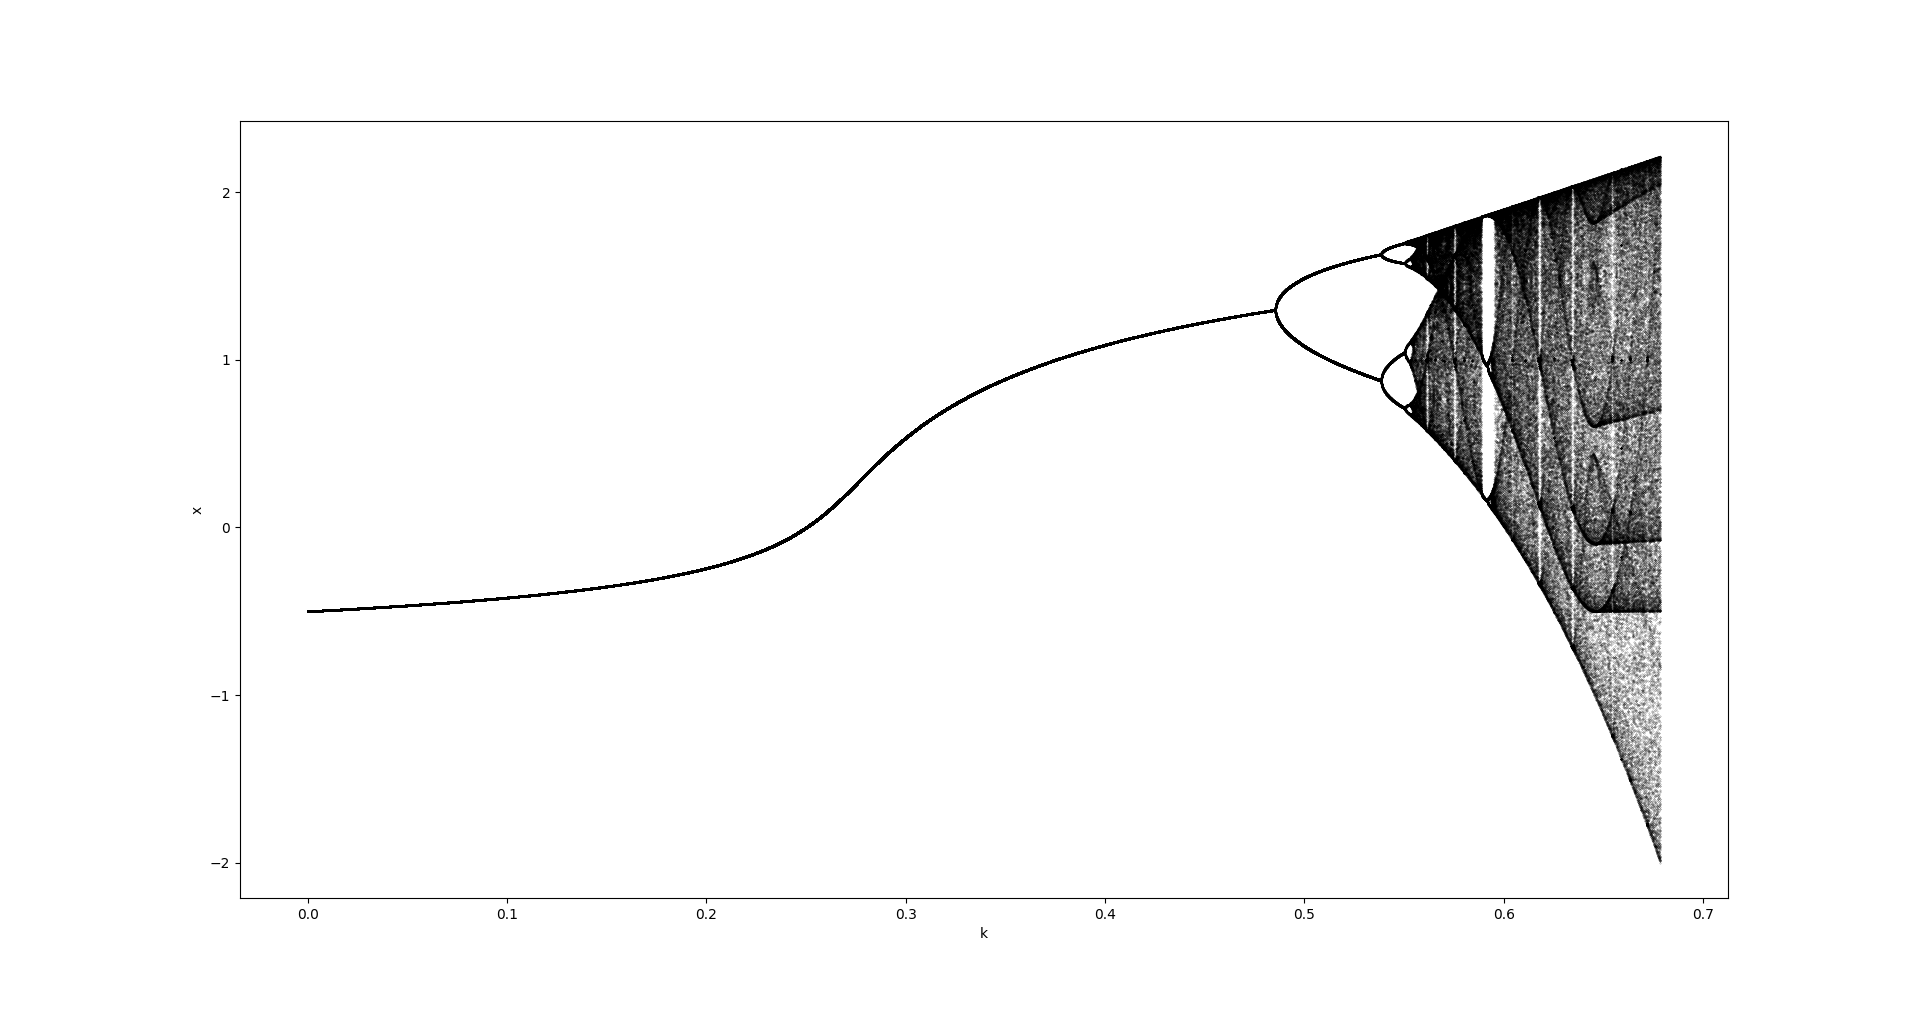
\includegraphics[width=0.8\linewidth]{LateX images/graphs q05/g1}
	\caption{ Διάγραμμα διακλάδωσης, για a=1, b=2 και q=-0.5}
	\label{f:g10}
\end{figure}

\begin{figure}[h!]
	\centering
	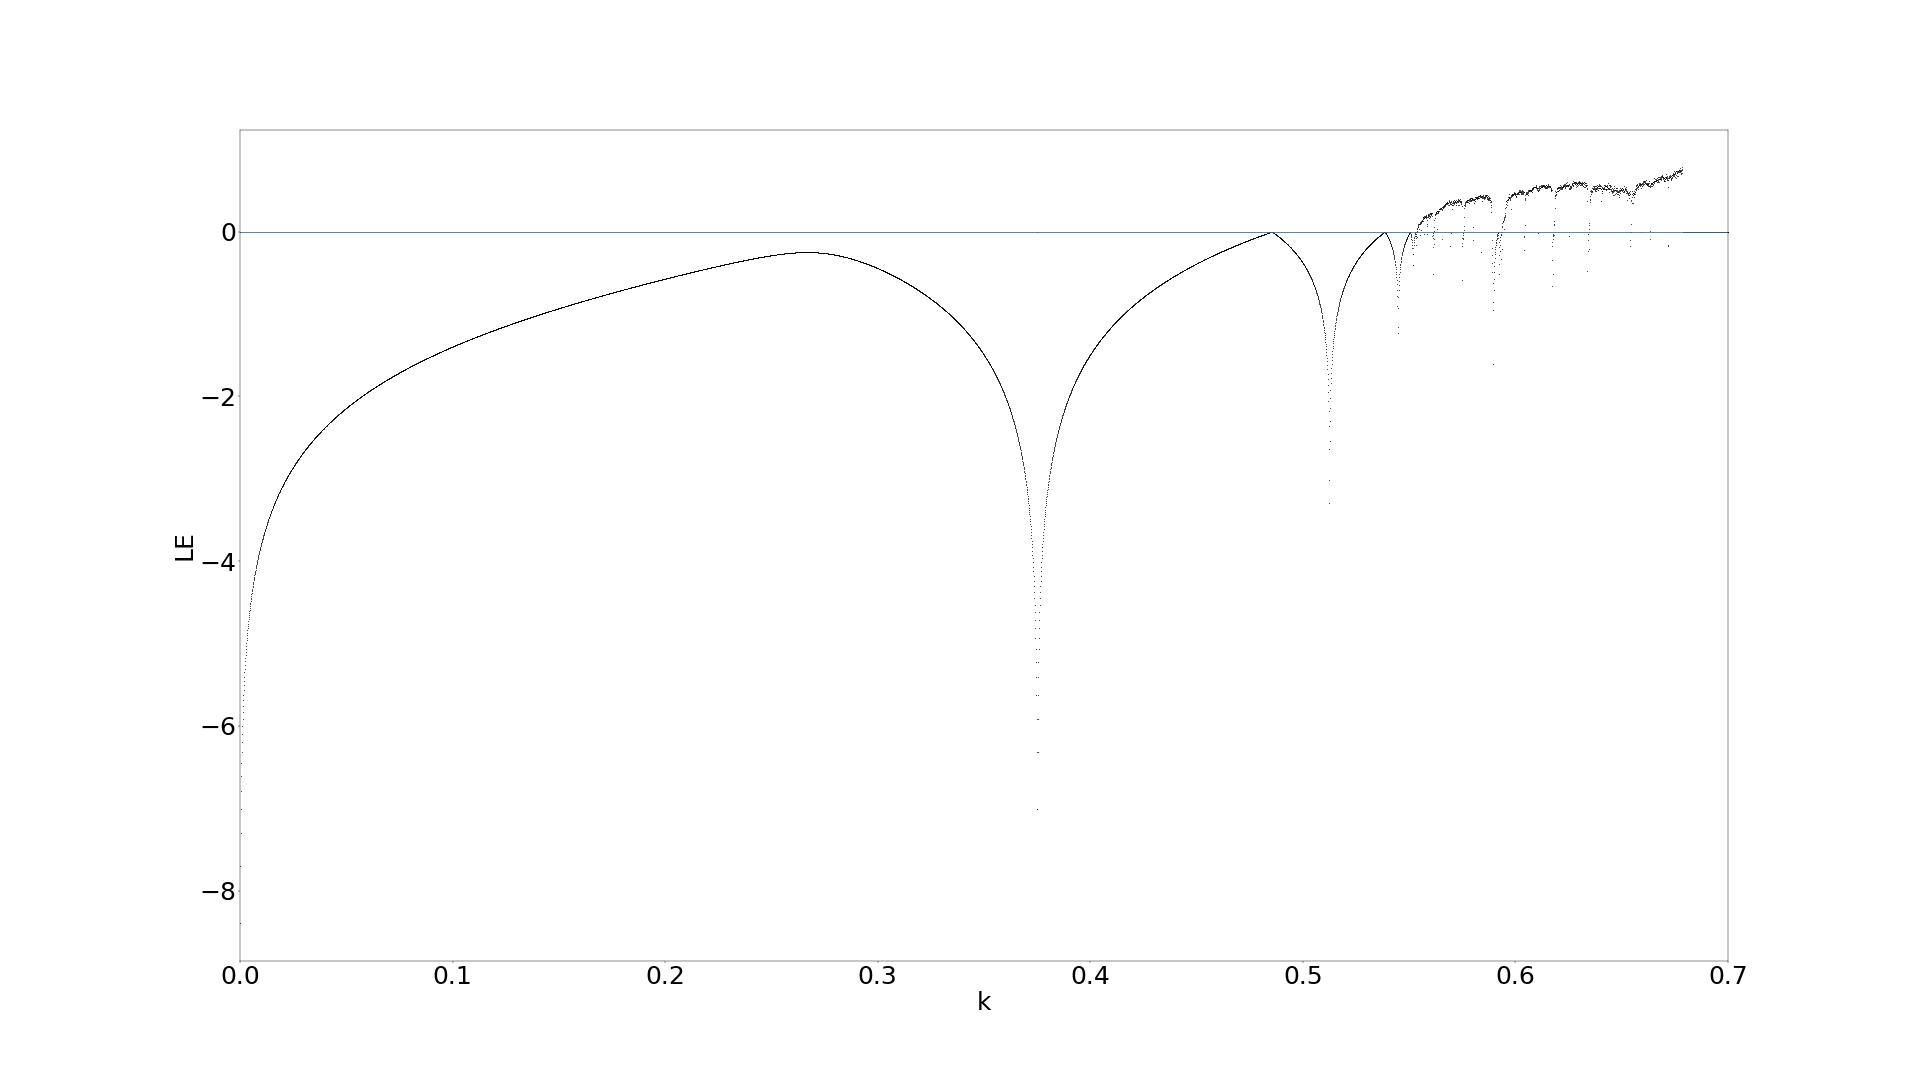
\includegraphics[width=0.6\linewidth]{LateX images/graphs q05/g2}
	\caption{ Διάγραμμα του εκθέτη Lyapunov σε συνάρτηση με την παράμετρο k, για a=1, b=2 και q=-0.5}
	\label{f:g11}
\end{figure}

\begin{figure}[h!]
	\centering
	\begin{subfigure}[b]{0.4\textwidth}
		\centering
		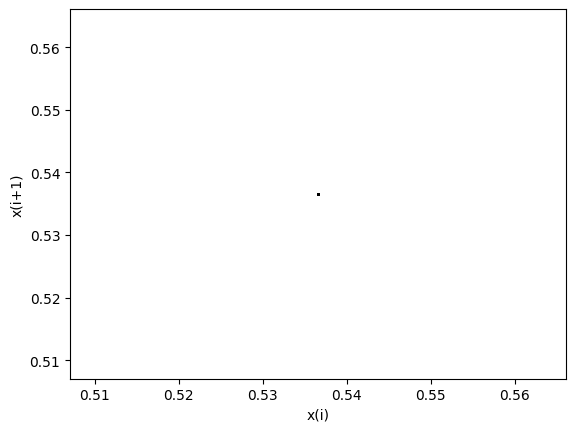
\includegraphics[width=\textwidth]{LateX images/graphs q05/g3}
		\caption{Για k=0.3}
		\label{f:k27}
	\end{subfigure}
	\hfill
	\begin{subfigure}[b]{0.4\textwidth}
		\centering
		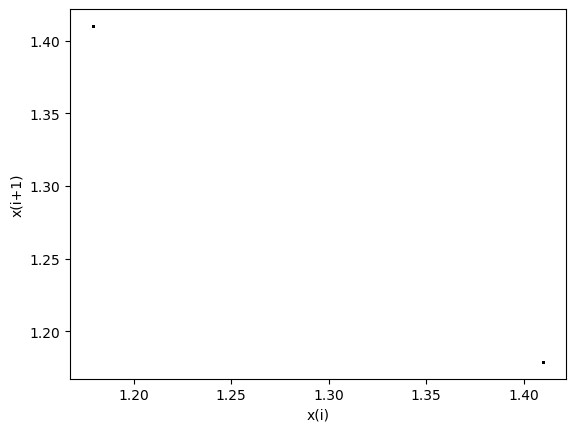
\includegraphics[width=\textwidth]{LateX images/graphs q05/g4}
		\caption{Για k=0.48}
		\label{f:k28}
	\end{subfigure}
	\hfill
	\begin{subfigure}[b]{0.4\textwidth}
		\centering
		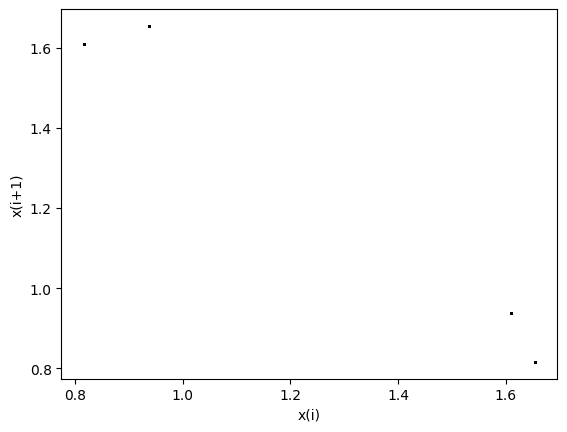
\includegraphics[width=\textwidth]{LateX images/graphs q05/g5}
		\caption{Για k=0.53}
		\label{f:k29}
	\end{subfigure}
	\hfill
	\begin{subfigure}[b]{0.4\textwidth}
		\centering
		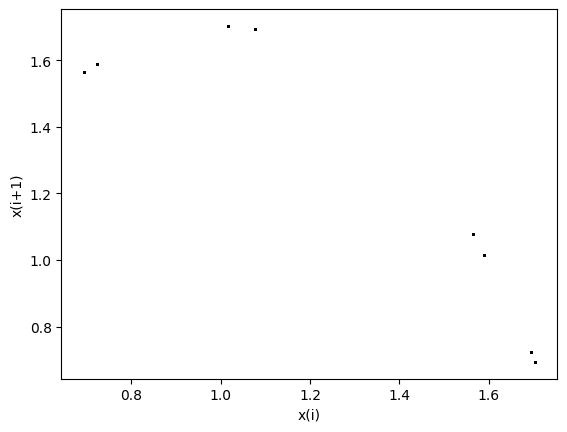
\includegraphics[width=\textwidth]{LateX images/graphs q05/g6}
		\caption{Για k=0.55}
		\label{f:k30}
	\end{subfigure}
	\hfill
	\caption{Διαγράμματα της τιμής \(x_i\) με την τιμή \(x_{i+1}\) α'μέρος :}
\end{figure}
\begin{figure}[h!]
	\begin{subfigure}[b]{0.4\textwidth}
		\centering
		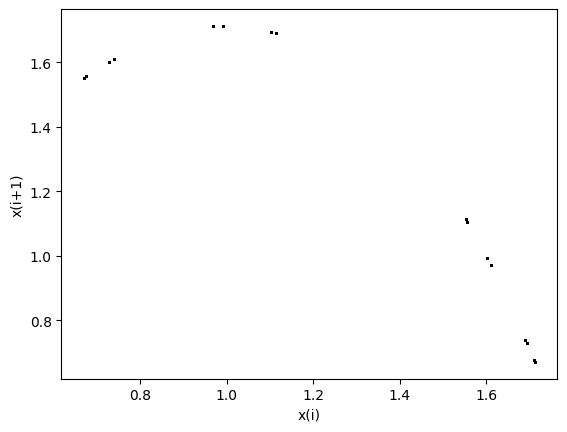
\includegraphics[width=\textwidth]{LateX images/graphs q05/g7}
		\caption{Για k=0.5531}
		\label{f:k31}
	\end{subfigure}
	\hfill
	\begin{subfigure}[b]{0.4\textwidth}
		\centering
		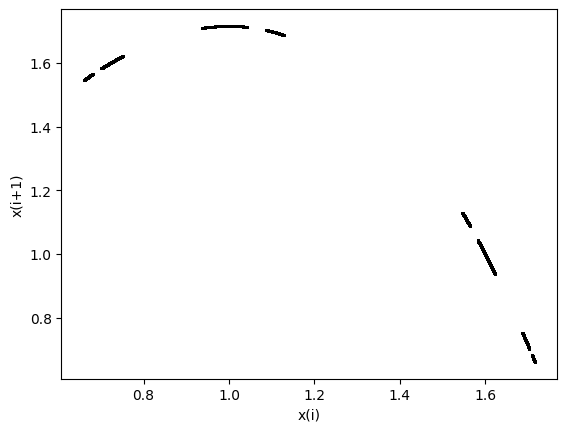
\includegraphics[width=\textwidth]{LateX images/graphs q05/g8}
		\caption{Για k=0.5534}
		\label{f:k32}
	\end{subfigure}
	\hfill
	\begin{subfigure}[c]{0.4\textwidth}
		\centering
		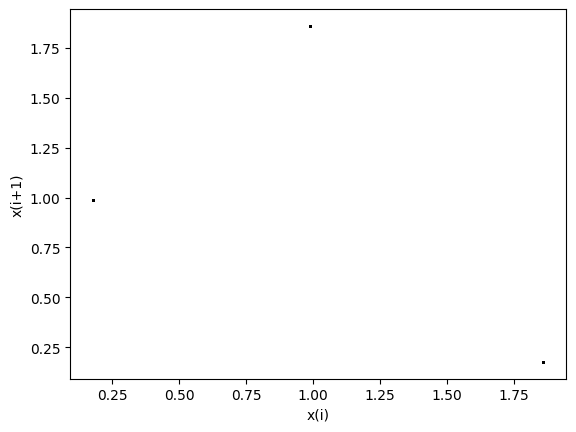
\includegraphics[width=\textwidth]{LateX images/graphs q05/g9}
		\caption{Για k=0.58}
		\label{f:k33}
	\end{subfigure}
	\hfill
	\begin{subfigure}[c]{0.4\textwidth}
		\centering
		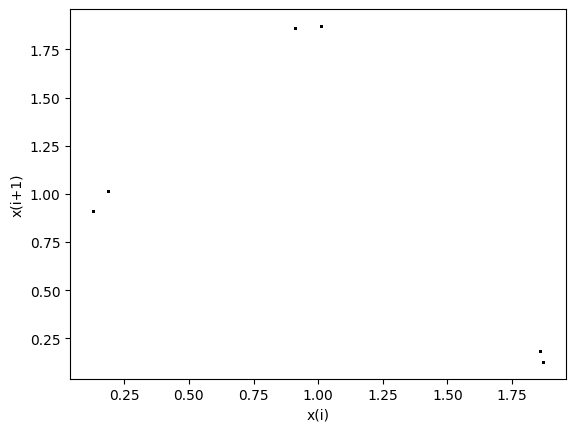
\includegraphics[width=\textwidth]{LateX images/graphs q05/g10}
		\caption{Για k=0.591}
		\label{f:k35}
	\end{subfigure}
	\hfill
	\begin{subfigure}[b]{0.4\textwidth}
		\centering
		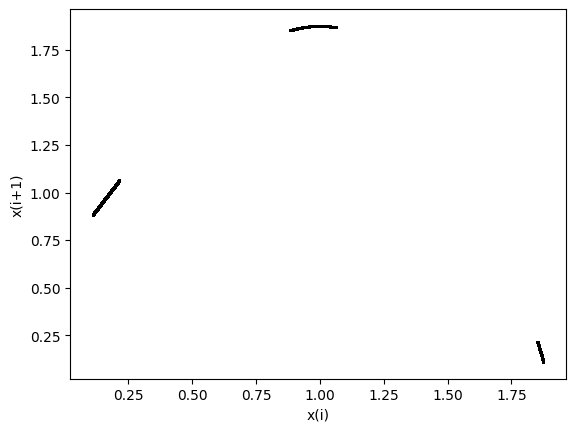
\includegraphics[width=\textwidth]{LateX images/graphs q05/g11}
		\caption{Για k=0.5927}
		\label{f:36}
	\end{subfigure}
	\hfill
\caption{Διαγράμματα της τιμής \(x_i\) με την τιμή \(x_{i+1}\) β´μέρος:}		
\end{figure}

 \clearpage

\subsection{Για q=-0.7}

Στο σχήμα \ref{f:g12} παρατίθεται το διάγραμμα διακλάδωσης του συστήματος \ref{f:x1}, ως προς την παράμετρο k, για a=1, b=2 και q =- 0.7. Για αυτές τις τιμές των παραμέτρων το σύστημα ξεκινάει από περίοδο-1 για k = 0.3 αλλά από k[0.3469,0.3486] "σπάει" η περίοδος.Αυτό το φαινόμενο αναφέρεται σαν υστέρηση και το κομμάτι όπου "σπάει" η περίοδος ονομάζεται βρόχός υστέρησης. Απο k=3.469 ξαναξεκινάει από περίοδο-1.Για  k = 0.52 εμφανίζει τον πρώτο διπλασιασμό της περιόδου. Τον δεύτερο διπλασιασμό τον εμφανίζει για k=0.57(περίοδος-4) ,τον τρίτο για k=0.592 (περίοδος-8) και τον τέταρτο για k=0.593(περόδος-15).Στην συνέχεια για k>0.593 το σύστημα εισέρχεται στο χάος , μέχρι να εξέλθει  για k=0.627(περίοδος-3) και να ξανά εισέλθει σε χάος μετά από δύο διπλασιασμούς k=0.63 (περίοδος-6)  k=0.631 (περίοδος-11),για k>0.631.
Επομένως και σε αυτή την περίπτωση το σύστημα εισέρχεται στο χάος με διπλασιασμό της περιόδου. 
Επιπλέον, στο σχήμα \ref{f:g11} παρατίθεται το διάγραμμα των εκθετών Lyapunov για τιμές του k στο ίδιο διάστημα τιμών [0, 0.72].  Στο διάστημα τιμών   0<k<0.594 , στο 0.627<k<0.632, παρατηρούμε ότι ο εκθέτης Lyapunov είναι συνεχώς αρνητικός, γεγονός που επιβεβαιώνει την περιοδική συμπεριφορά του συστήματος. Ενώ στα υπόλοιπα διαστήματα ο θετικός εκθέτης Lyapunov υποστηρίζει την χαοτική του συμπεριφορά, όπως έγινε φανερό και από το διάγραμμα διακλάδωσης.
Τέλος, στον Πίνακα \ref{tab:abc3} παρατίθενται ενδεικτικές τιμές της παραμέτρου k και η συμπεριφορά που παρουσιάζει το σύστημα για αυτές, σύμφωνα με το διάγραμμα διακλάδωσης, καθώς και τα αντίστοιχα σχήματα των διαγραμμάτων της τιμής \(x_i\) σε συνάρτηση με την τιμή \(x_{i+1}\). Από τα παραγόμενα σχήματα προκύπτει αριθμός σημείων αντίστοιχος με την περίοδο του συστήματος.

\begin{table}[h!]
	\centering
	\begin{tabular}{l | l | l}
		Παράμετρος k & Συμπεριφορά & Σχήμα\\
		\hline
		0.25 &  Περίοδος-1 & \ref{f:k37}\\
		0.3469&  Περίοδος-1 & \ref{f:k38}\\
		0.52& Περίοδος-2 & \ref{f:k39}\\
		0.57& Περίοδος-4 & \ref{f:k40}\\
		0.592 &  Περίοδος-8 & \ref{f:k41}\\
		0.593& Περίοδος-15 & \ref{f:k42}\\
		0.594 & Χάος & \ref{f:k43}\\
		0.627 & Περίοδος-3 & \ref{f:k44}\\
		0.630 & Περίοδος-6 & \ref{f:k45}\\
		0.631 & Περίοδος-11 & \ref{f:k46}\\
		0.632 & Χάος & \ref{f:k47}\\
	\end{tabular}
	\caption{ Συμπεριφορά του υπό μελέτη συστήματος για διάφορες τιμές του k,για a=1, b=2 και q=-0.7}
	\label{tab:abc3}
\end{table}

\begin{figure}[h!]
	\centering
	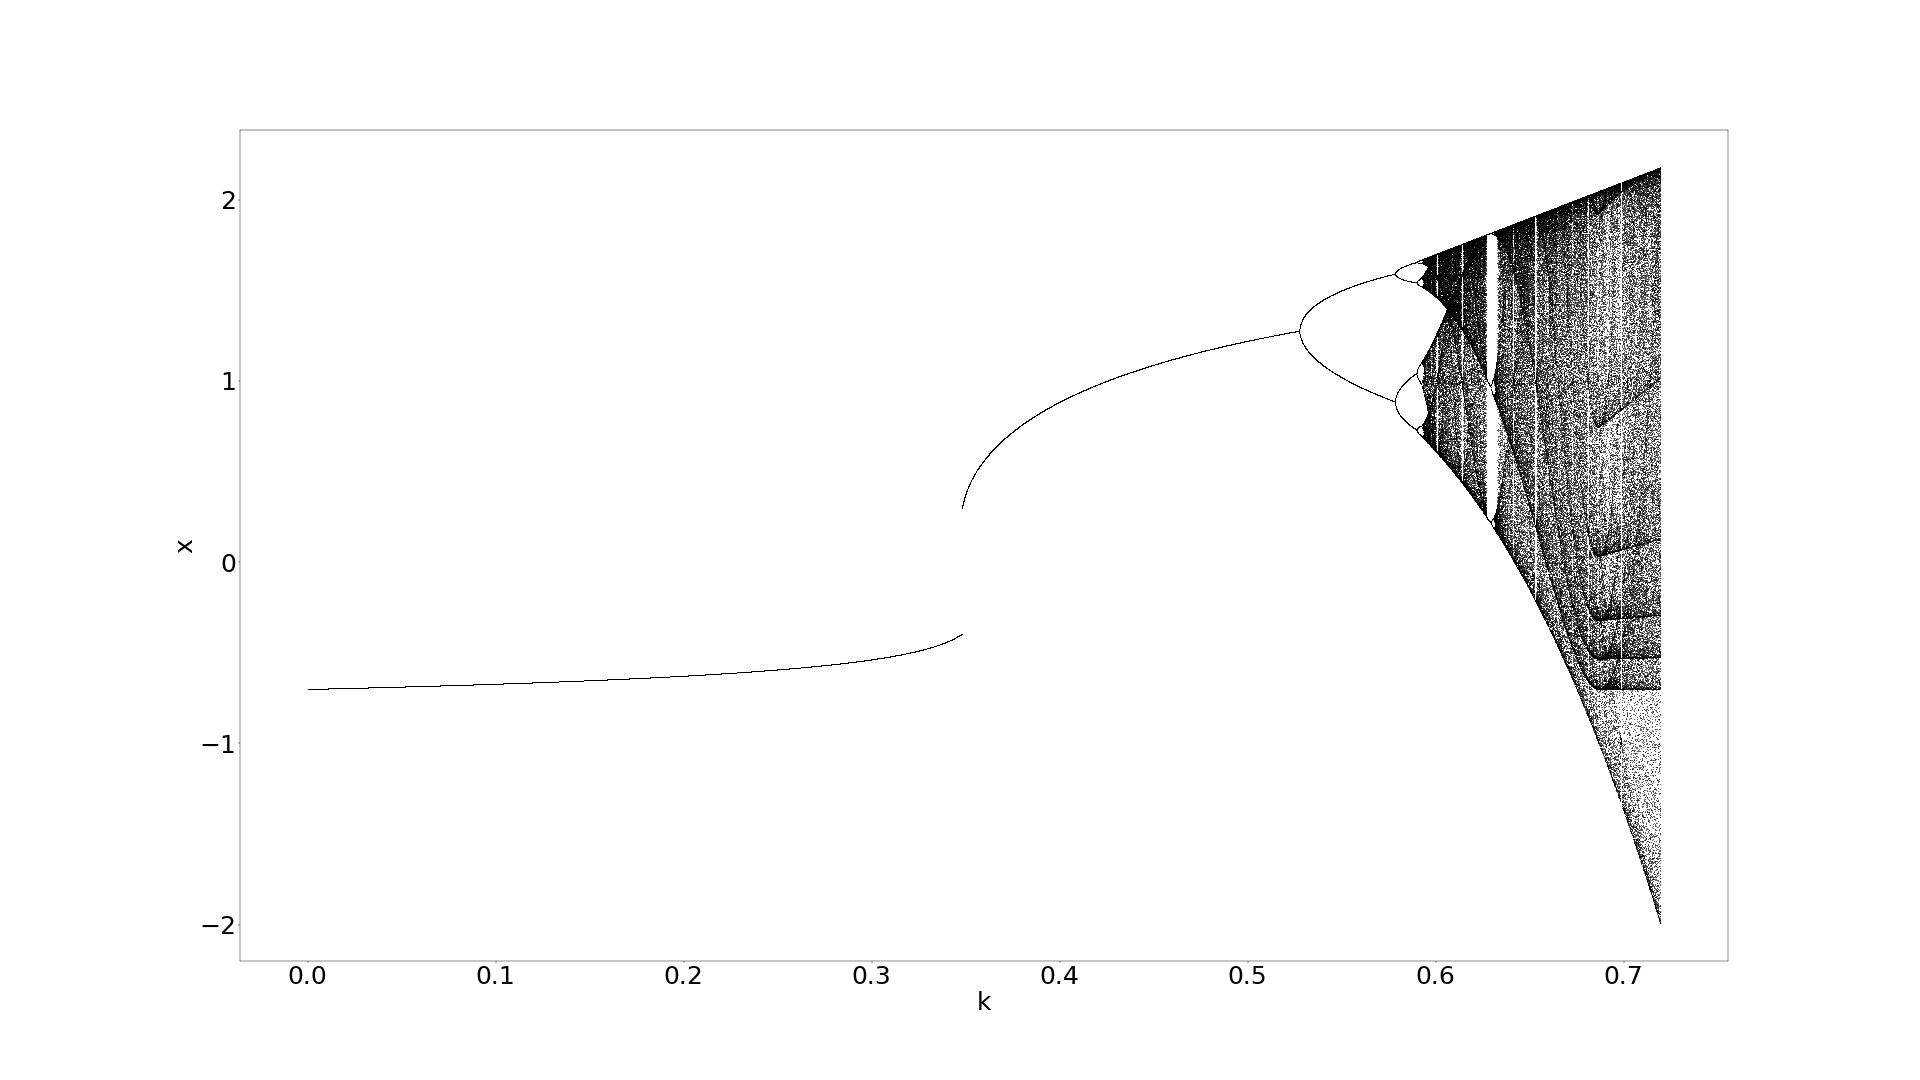
\includegraphics[width=0.8\linewidth]{LateX images/graphs q07/g1}
	\caption{ Διάγραμμα διακλάδωσης, για a=1, b=2 και q=-0.7}
	\label{f:g12}
\end{figure}
\begin{figure}[h!]
	\centering
	\includegraphics[width=0.6\linewidth]{"LateX images/graphs q07/g2 "}
	\caption{Διάγραμμα του εκθέτη Lyapunov σε συνάρτηση με την παράμετρο k, για a=1, b=2 και q=-0.7.}
	\label{f:g13}
\end{figure}

\begin{figure}[h!]
	\centering
	
	\begin{subfigure}[b]{0.4\textwidth}
		\centering
		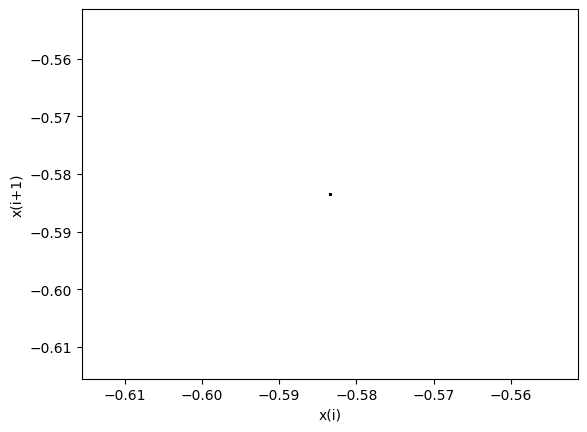
\includegraphics[width=\textwidth]{LateX images/graphs q07/g3}
		\caption{Για k=0.25}
		\label{f:k37}
	\end{subfigure}
	\hfill
	\begin{subfigure}[b]{0.4\textwidth}
		\centering
		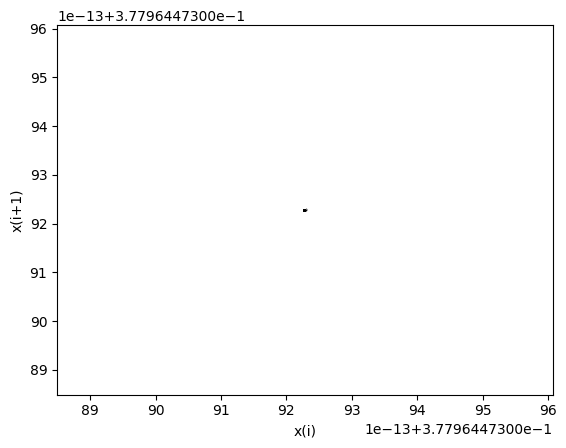
\includegraphics[width=\textwidth]{LateX images/graphs q07/g4}
		\caption{Για k=0.3469}
		\label{f:k38}
	\end{subfigure}
	\hfill
	\begin{subfigure}[b]{0.4\textwidth}
		\centering
		\includegraphics[width=\textwidth]{LateX images/graphs q07/g5}
		\caption{Για k=0.52}
		\label{f:k39}
	\end{subfigure}
	\hfill
	\begin{subfigure}[b]{0.4\textwidth}
		\centering
		\includegraphics[width=\textwidth]{LateX images/graphs q07/g6}
		\caption{Για k=0.57}
		\label{f:k40}
	\end{subfigure}
	\hfill
	\begin{subfigure}[b]{0.4\textwidth}
		\centering
		\includegraphics[width=\textwidth]{LateX images/graphs q07/g7}
		\caption{Για k=0.592}
		\label{f:k41}
	\end{subfigure}
	\hfill
	\caption{Διαγράμματα της τιμής \(x_i\) με την τιμή \(x_{i+1}\) α'μέρος :}
\end{figure}
\begin{figure}[h!]
\centering
	\begin{subfigure}[b]{0.4\textwidth}
		\centering
		\includegraphics[width=\textwidth]{LateX images/graphs q07/g8}
		\caption{Για k=0.593}
		\label{f:k42}
	\end{subfigure}
	\hfill
	\begin{subfigure}[b]{0.4\textwidth}
		\centering
		\includegraphics[width=\textwidth]{LateX images/graphs q07/g9}
		\caption{Για k=0.594}
		\label{f:k43}
	\end{subfigure}
	\hfill
	\begin{subfigure}[b]{0.4\textwidth}
		\centering
		\includegraphics[width=\textwidth]{LateX images/graphs q07/g10}
		\caption{Για k=0.627}
		\label{f:k44}
	\end{subfigure}
	\hfill
	\begin{subfigure}[b]{0.4\textwidth}
		\centering
		\includegraphics[width=\textwidth]{LateX images/graphs q07/g11}
		\caption{Για k=0.63}
		\label{f:k45}
	\end{subfigure}
	\hfill
	\begin{subfigure}[b]{0.4\textwidth}
		\centering
		\includegraphics[width=\textwidth]{LateX images/graphs q07/g12}
		\caption{Για k=0.631}
		\label{f:k46}
	\end{subfigure}
	\hfill
	\begin{subfigure}[b]{0.4\textwidth}
	\centering
	\includegraphics[width=\textwidth]{LateX images/graphs q07/g13}
	\caption{Για k=0.632}
	\label{f:k47}
	\end{subfigure}
\caption{Διαγράμματα της τιμής \(x_i\) με την τιμή \(x_{i+1}\) β'μέρος :}	
\end{figure}

\clearpage

\subsection{Για q=-0.9}

Στο σχήμα \ref{f:g14} παρατίθεται το διάγραμμα διακλάδωσης του συστήματος \ref{f:x1}, ως προς την παράμετρο k, για a=1, b=2 και q =- 0.9. Για αυτές τις τιμές των παραμέτρων το σύστημα ξεκινάει από περίοδο-1 για k = 0.3 αλλά από k[0.43,0.436] "σπάει" η περίοδος.Αυτό το φαινόμενο αναφέρεται σαν υστέρηση και το κομμάτι όπου "σπάει" η περίοδος ονομάζεται βρόχός υστέρησης. Απο k=3.436 ξαναξεκινάει από περίοδο-1.Για  k = 0.57 εμφανίζει τον πρώτο διπλασιασμό της περιόδου. Τον δεύτερο διπλασιασμό τον εμφανίζει για k=0.62 (περίοδος-4) ,τον τρίτο για k=0.63 (περίοδος-8) και τον τέταρτο για k=0.633(περόδος-16).Στην συνέχεια για k>0.635 το σύστημα εισέρχεται στο χάος , μέχρι να εξέλθει  για k=0.665 (περίοδος-3) και να ξανά εισέλθει σε χάος μετά από ένα διπλασιασμό k=0.668 (περίοδος-6),για k>0.671.Παρόλα αυτά παρατηρέιται μία ακόμα έξοδος απο το χάος για k=0.72(περίοδος-1).
Για q=-0.9 το σύστημα εισέρχεται στο χάος με διπλασιασμό της περιόδου.
Επιπλέον, στο σχήμα \ref{f:g15} παρατίθεται το διάγραμμα των εκθετών Lyapunov για τιμές του k στο ίδιο διάστημα τιμών [0, 0.77].  Στο διάστημα τιμών   0<k<0.635 , στο 0.665<k<0.671 καί 0.72<k<0.77 παρατηρούμε ότι ο εκθέτης Lyapunov είναι συνεχώς αρνητικός, γεγονός που επιβεβαιώνει την περιοδική συμπεριφορά του συστήματος. Ενώ στα υπόλοιπα διαστήματα ο θετικός εκθέτης Lyapunov υποστηρίζει την χαοτική του συμπεριφορά, όπως έγινε φανερό και από το διάγραμμα διακλάδωσης.
Τέλος, στον Πίνακα \ref{tab:abc4} παρατίθενται ενδεικτικές τιμές της παραμέτρου k και η συμπεριφορά που παρουσιάζει το σύστημα για αυτές, σύμφωνα με το διάγραμμα διακλάδωσης, καθώς και τα αντίστοιχα σχήματα των διαγραμμάτων της τιμής \(x_i\) σε συνάρτηση με την τιμή \(x_{i+1}\). Από τα παραγόμενα σχήματα προκύπτει αριθμός σημείων αντίστοιχος με την περίοδο του συστήματος.

\begin{table}[h!]
	\centering
	\begin{tabular}{l | l | l}
		Παράμετρος k & Συμπεριφορά & Σχήμα\\
		\hline
		0.43 &  Περίοδος-1 & \ref{f:k48}\\
		0.436 &  Περίοδος-1 & \ref{f:k49}\\
		0.57& Περίοδος-2 & \ref{f:k50}\\
		0.62& Περίοδος-4 & \ref{f:k51}\\
		0.63 &  Περίοδος-8 & \ref{f:k52}\\
		0.633& Περίοδος-16 & \ref{f:k53}\\
		0.635& Χάος & \ref{f:k54}\\
		0.665 & Περίοδος-3 & \ref{f:k55}\\
		0.668 & Περίοδος-6 & \ref{f:k56}\\
		0.671 & Χάος & \ref{f:k57}\\
		0.72 & Περίοδος-1& \ref{f:k58}\\
	\end{tabular}
	\caption{ Συμπεριφορά του υπό μελέτη συστήματος για διάφορες τιμές του k,για a=1, b=2 και q=-0.9}
	\label{tab:abc4}
\end{table}

\begin{figure}[h!]
	\centering
	\includegraphics[width=0.8\linewidth]{LateX images/graphs q09/g1}
	\caption{ Διάγραμμα διακλάδωσης, για a=1, b=2 και q=-0.9}
	\label{f:g14}
\end{figure}

\begin{figure}[h!]
	\centering
	\includegraphics[width=0.6\linewidth]{LateX images/graphs q09/g2}
	\caption{Διάγραμμα του εκθέτη Lyapunov σε συνάρτηση με την παράμετρο k, για a=1, b=2 και q=-0.9}
	\label{f:g15}
\end{figure}

\begin{figure}[h!]
	\centering
	\begin{subfigure}[b]{0.4\textwidth}
		\centering
		\includegraphics[width=\textwidth]{LateX images/graphs q09/g3}
		\caption{Για k=0.43}
		\label{f:k48}
	\end{subfigure}
	\hfill
	\begin{subfigure}[b]{0.4\textwidth}
		\centering
		\includegraphics[width=\textwidth]{LateX images/graphs q09/g4}
		\caption{Για k=0.436}
		\label{f:k49}
	\end{subfigure}
	\hfill
	\begin{subfigure}[b]{0.4\textwidth}
		\centering
		\includegraphics[width=\textwidth]{LateX images/graphs q09/g5}
		\caption{Για k=0.57}
		\label{f:k50}
	\end{subfigure}
\hfill
	\begin{subfigure}[b]{0.4\textwidth}
		\centering
		\includegraphics[width=\textwidth]{LateX images/graphs q09/g6}
		\caption{Για k=0.62}
		\label{f:k51}
	\end{subfigure}
	\hfill
	\begin{subfigure}[b]{0.4\textwidth}
		\centering
		\includegraphics[width=\textwidth]{LateX images/graphs q09/g13}
		\caption{Για k=0.63}
		\label{f:k52}
	\end{subfigure}
	\hfill
	\caption{Διαγράμματα της τιμής \(x_i\) με την τιμή \(x_{i+1}\) α'μέρος:}
\end{figure}
\begin{figure}
	\centering
	\begin{subfigure}[b]{0.4\textwidth}
		\centering
		\includegraphics[width=\textwidth]{LateX images/graphs q09/g7}
		\caption{Για k=0.633}
		\label{f:k53}
	\end{subfigure}
	\hfill
	\begin{subfigure}[b]{0.4\textwidth}
		\centering
		\includegraphics[width=\textwidth]{LateX images/graphs q09/g8}
		\caption{Για k=0.635}
		\label{f:k54}
	\end{subfigure}
	\hfill
	\begin{subfigure}[b]{0.4\textwidth}
		\centering
		\includegraphics[width=\textwidth]{LateX images/graphs q09/g9}
		\caption{Για k=0.665}
		\label{f:k55}
	\end{subfigure}
	\hfill
	\begin{subfigure}[b]{0.4\textwidth}
		\centering
		\includegraphics[width=\textwidth]{LateX images/graphs q09/g10}
		\caption{Για k=0.668}
		\label{f:k56}
	\end{subfigure}
	\hfill
	\begin{subfigure}[b]{0.4\textwidth}
		\centering
		\includegraphics[width=\textwidth]{LateX images/graphs q09/g11}
		\caption{Για k=0.671}
		\label{f:k57}
	\end{subfigure}
	\hfill
	\begin{subfigure}[b]{0.4\textwidth}
		\centering
		\includegraphics[width=\textwidth]{LateX images/graphs q09/g12}
		\caption{Για k=0.72}
		\label{f:k58}
	\end{subfigure}
	\hfill
	\caption{Διαγράμματα της τιμής \(x_i\) με την τιμή \(x_{i+1}\) β'μέρος:}
\end{figure}

\clearpage

\subsection{Για q=-1.2}
Στο σχήμα \ref{f:g16} παρατίθεται το διάγραμμα διακλάδωσης του συστήματος \ref{f:x1}, ως προς την παράμετρο k, για a=1, b=2 και q =- 1.2. Για αυτές τις τιμές των παραμέτρων το σύστημα ξεκινάει από περίοδο-1 για k = 0.55 αλλά από k[0.56,0.566] "σπάει" η περίοδος.Αυτό το φαινόμενο αναφέρεται σαν υστέρηση και το κομμάτι όπου "σπάει" η περίοδος ονομάζεται βρόχός υστέρησης. Απο k=0.566 ξαναξεκινάει από περίοδο-1.Για  k = 0.63 εμφανίζει τον πρώτο διπλασιασμό της περιόδου. Τον δεύτερο διπλασιασμό τον εμφανίζει για k=0.67 (περίοδος-4) και τον τρίτο για k=0.69 (περίοδος-8) .Στην συνέχεια για k>0.696 το σύστημα εισέρχεται στο χάος,μέχρι να εξέλθει  για k=0.726 (περίοδος-3) και να ξανά εισέλθει σε χάος μετά από ένα διπλασιασμό k=0.729 (περίοδος-6),για k>0.731.Παρόλα αυτά παρατηρέιται μία ακόμα έξοδος απο το χάος για k=0.762(περίοδος-1).
Για q=-1.2το σύστημα εισέρχεται στο χάος με διπλασιασμό της περιόδου,ενώ παρατηρείται και εσωτερική κρίση ελκυστή για k=0.726 αλλά και για k=0.762
Επιπλέον, στο σχήμα \ref{f:g17} παρατίθεται το διάγραμμα των εκθετών Lyapunov για τιμές του k στο ίδιο διάστημα τιμών [0, 0.77].  Στο διάστημα τιμών   0<k<0.69 , στο 0.726<k<0.731 καί 0.72<k<0.8574 παρατηρούμε ότι ο εκθέτης Lyapunov είναι συνεχώς αρνητικός, γεγονός που επιβεβαιώνει την περιοδική συμπεριφορά του συστήματος. Ενώ στα υπόλοιπα διαστήματα ο θετικός εκθέτης Lyapunov υποστηρίζει την χαοτική του συμπεριφορά, όπως έγινε φανερό και από το διάγραμμα διακλάδωσης.
Τέλος, στον Πίνακα \ref{tab:abc5} παρατίθενται ενδεικτικές τιμές της παραμέτρου k και η συμπεριφορά που παρουσιάζει το σύστημα για αυτές, σύμφωνα με το διάγραμμα διακλάδωσης, καθώς και τα αντίστοιχα σχήματα των διαγραμμάτων της τιμής \(x_i\) σε συνάρτηση με την τιμή \(x_{i+1}\). Από τα παραγόμενα σχήματα προκύπτει αριθμός σημείων αντίστοιχος με την περίοδο του συστήματος.
\begin{table}[h!]
	\centering
	\begin{tabular}{l | l | l}
		Παράμετρος k & Συμπεριφορά & Σχήμα\\
		\hline
		0.55 &  Περίοδος-1 & \ref{f:k59}\\
		0.566 &  Περίοδος-1 & \ref{f:k60}\\
		0.63& Περίοδος-2 & \ref{f:k61}\\
		0.68& Περίοδος-4 & \ref{f:k62}\\
		0.69 &  Περίοδος-8 & \ref{f:k63}\\
		0.696& Χάος & \ref{f:k64}\\
		0.726& Περίοδος-3 & \ref{f:k65}\\
		0.729& Περίοδος-6 & \ref{f:k66}\\
		0.731& Χάος & \ref{f:k67}\\
		0.762 &  Περίοδος-1 & \ref{f:k68}\\
	\end{tabular}
	\caption{ Συμπεριφορά του υπό μελέτη συστήματος για διάφορες τιμές του k,για a=1, b=2 και q=-0.9}
	\label{tab:abc5}
\end{table}

\begin{figure}[h!]
	\centering
	\includegraphics[width=0.8\linewidth]{LateX images/graphs q12/g1}
	\caption{ Διάγραμμα διακλάδωσης, για a=1, b=2 και q=-1.2}
	\label{f:g16}
\end{figure}

\begin{figure}[h!]
	\centering
	\includegraphics[width=0.6\linewidth]{LateX images/graphs q12/g2}
	\caption{Διάγραμμα του εκθέτη Lyapunov σε συνάρτηση με την παράμετρο k, για a=1, b=2 και q=-1.2}
	\label{f:g17}
\end{figure}

\begin{figure}[h!]
	\centering
	
	\begin{subfigure}[b]{0.4\textwidth}
		\centering
		\includegraphics[width=\textwidth]{LateX images/graphs q12/g3}
		\caption{Για k=0.55}
		\label{f:k59}
	\end{subfigure}
	\hfill
	\begin{subfigure}[b]{0.4\textwidth}
		\centering
		\includegraphics[width=\textwidth]{LateX images/graphs q12/g4}
		\caption{Για k=0.566}
		\label{f:k60}
	\end{subfigure}
	\hfill
	\begin{subfigure}[b]{0.4\textwidth}
		\centering
		\includegraphics[width=\textwidth]{LateX images/graphs q12/g5}
		\caption{Για k=0.63}
		\label{f:k61}
	\end{subfigure}
	\hfill
	\begin{subfigure}[b]{0.4\textwidth}
		\centering
		\includegraphics[width=\textwidth]{LateX images/graphs q12/g6}
		\caption{Για k=0.68}
		\label{f:k62}
	\end{subfigure}
	\hfill
	\begin{subfigure}[b]{0.4\textwidth}
		\centering
		\includegraphics[width=\textwidth]{LateX images/graphs q12/g7}
		\caption{Για k=0.69}
		\label{f:k63}
	\end{subfigure}
	\hfill
	\begin{subfigure}[b]{0.4\textwidth}
		\centering
		\includegraphics[width=\textwidth]{LateX images/graphs q12/g8}
		\caption{Για k=0.696}
		\label{f:k64}
	\end{subfigure}
	\hfill
	\caption{Διαγράμματα της τιμής \(x_i\) με την τιμή \(x_{i+1}\) α'μέρος :}
\end{figure}
\begin{figure}[h!]
	\centering
	\begin{subfigure}[b]{0.4\textwidth}
		\centering
		\includegraphics[width=\textwidth]{LateX images/graphs q12/g9}
		\caption{Για k=0.726}
		\label{f:k65}
	\end{subfigure}
	\hfill
	\begin{subfigure}[b]{0.4\textwidth}
		\centering
		\includegraphics[width=\textwidth]{LateX images/graphs q12/g10}
		\caption{Για k=0.729}
		\label{f:k66}
	\end{subfigure}
	\hfill
	\begin{subfigure}[b]{0.4\textwidth}
		\centering
		\includegraphics[width=\textwidth]{LateX images/graphs q12/g11}
		\caption{Για k=0.731}
		\label{f:k67}
	\end{subfigure}
	\hfill
	\begin{subfigure}[b]{0.4\textwidth}
		\centering
		\includegraphics[width=\textwidth]{LateX images/graphs q12/g12}
		\caption{Για k=0.762}
		\label{f:k68}
	\end{subfigure}
	\hfill
\caption{Διαγράμματα της τιμής \(x_i\) με την τιμή \(x_{i+1}\) β'μέρος :}	
\end{figure}

\clearpage

\subsection{Για q=-1.4}
Στο σχήμα \ref{f:g233} παρατίθονται τα διαγράμματα διακλάδωσης του συστήματος \ref{f:x1}, ως προς την παράμετρο k, για a=1, b=2 ,q =- 1.4 και για διαφορετικές αρχικές συνθήκες δηλαδή για διαφορετικό \(x_0\). Συγκρίνοντας το διάγραμμα \ref{f:g19} (\(x_0=0.1\))με τα υπόλοιπα διαγράμματα διακλάδωσεις \ref{f:g20} (\(x_0=0.5\)), \ref{f:g21} (\(x_0=1\), \ref{f:g22} (\(x_0=-0.1\)) πατατηρείται ότι για q= -1.4 εμφανίζεται το φαινόμενο της συνύπαρξης ελκυστών.Αυτό το φαινόμενο επιβεβαιώνεται καί απο τα διαγράμματα Lyapunov \ref{f:g23} , \ref{f:g24},  \ref{f:g25},  \ref{f:g26} 
Στον Πίνακα \ref{tab:abc6} φαίνεται η πορεία του συστήματος και για ποιές τιμές της παραμέτρου  k το σύστημα εμφανίζει περιοδική συμπεριφορά ή χαοτική, σύμφωνα με το διάγραμμα διακλάδωσης \ref{f:g19}.Επίσης οι τιμές αυτές αντιστοιχόυν στα σχήματα των διαγραμματων της τιμή)ς \(x_i\) σε συνάρτηση με την τιμή \(x_{i+1}\).πό τα παραγόμενα σχήματα προκύπτει αριθμός σημείων αντίστοιχος με την περίοδο του συστήματος.
Επίσης παρατηρείται εσωτερκή κρίση ελκυστών για δίαφορες τιμές του k(0.744, 0.7565 , 0.768 , 0.8), όπως και το φαινόμενο της υστέρησης το οποίο φαίνεται στο διάγραμμα διακλάδωσης \ref{f:g19} στην μεταπήδηση του συστήματος από χαοτική συμπεριφορά σε περίοδο-2 ,αλλά και από περίοδο-2 σε περίοδο-1. Οι αντίστοιχες τιμές του k για αυτά τα σημεία του διαγράμματος υπάρχουν στο πίνακα \ref{tab:abc7}
Τέλος, στο σχήμα \ref{f:g23} παρατίθεται το διάγραμμα των εκθετών Lyapunov για τιμές του k στο ίδιο διάστημα τιμών [0, 0.91]. Οι τιμές του πίνακα \ref{tab:abc6} που έχουνε περιοδική συμπεριφορά αντιστοιχουν σε τιμές του διαγράμματος \ref{f:g23} όπου ο εκθέτης Lyapunov είναι συνεχώς αρνητικός, γεγονός που επιβεβαιώνει την συμπεριφορά τους Ενώ για τις υπόλοιπες τιμές ο θετικός εκθέτης Lyapunov υποστηρίζει την χαοτική τους συμπεριφορά, όπως έγινε φανερό και από το διάγραμμα διακλάδωσης.

\begin{table}[h!]
	\centering
	\begin{tabular}{l | l | l}
		Παράμετρος k & Συμπεριφορά & Σχήμα\\
		\hline
		0.4 &  Περίοδος-1 & \ref{f:k}\\
		0.54 &  Περίοδος-2 & \ref{f:k69}\\
		0.65& Περίοδος-1 & \ref{f:k70}\\
		0.68& Περίοδος-2 & \ref{f:k71}\\
		0.726 &  Περίοδος-4 & \ref{f:k72}\\
		0.737& Περίοδος-8 & \ref{f:k73}\\
		0.738& Περίοδος-15 & \ref{f:k74}\\
		0.739& Χάος & \ref{f:k75}\\
		0.744 &  Περίοδος-6 & \ref{f:k76}\\
		0.746 &  Χάος & \ref{f:k77}\\
		0.7565 &  Περίοδος-5 & \ref{f:k78}\\
		0.757 &  Χάος & \ref{f:k79}\\
		0.768 &  Περίοδος-3 & \ref{f:k83}\\
		0.77 &  Περίοδος-6 & \ref{f:k80}\\
		0.78 &  Χάος & \ref{f:k81}\\
		0.8 & Περίοδος-2&\ref{f:k82}\\
	\end{tabular}
	\caption{ Συμπεριφορά του υπό μελέτη συστήματος για διάφορες τιμές του k,για a=1, b=2 , q=-1.4 και
	\(x_i=0.1\)}
	\label{tab:abc6}
\end{table}

\begin{figure}[h!]
	\centering
	
	\begin{subfigure}[b]{0.7\textwidth}
		\centering
		\includegraphics[width=\textwidth]{LateX images/graphs q14/g1}
		\caption{\(x_0=0.1\)}
		\label{f:g19}
	\end{subfigure}
	\hfill
	\begin{subfigure}[b]{0.7\textwidth}
		\centering
		\includegraphics[width=\textwidth]{LateX images/graphs q14/g2}
		\caption{\(x_0=0.5\)¨}
		\label{f:g20}
	\end{subfigure}
	\hfill
	\begin{subfigure}[b]{0.7\textwidth}
		\centering
		\includegraphics[width=\textwidth]{LateX images/graphs q14/g3}
		\caption{\(x_0=1\)}
		\label{f:g21}
	\end{subfigure}
	\hfill
	\begin{subfigure}[b]{0.7\textwidth}
		\centering
		\includegraphics[width=\textwidth]{LateX images/graphs q14/g5}
		\caption{\(x_0=-0.1\)}
		\label{f:g22}
	\end{subfigure}
	\hfill
	\caption{ Διάγραμμα διακλάδωσης, για a=1, b=2, q=-1.4 και για:}
\end{figure}

\begin{figure}[h!]
	\centering

	\begin{subfigure}[b]{0.45\textwidth}
		\centering
		\includegraphics[width=\textwidth]{LateX images/graphs q14/g6}
		\caption{\(x_0=0.1\)}
		\label{f:g23}
	\end{subfigure}
	\hfill
	\begin{subfigure}[b]{0.45\textwidth}
		\centering
		\includegraphics[width=\textwidth]{LateX images/graphs q14/g7}
		\caption{\(x_0=0.5\)¨}
		\label{f:g24}
	\end{subfigure}
	\hfill
	\begin{subfigure}[b]{0.45\textwidth}
		\centering
		\includegraphics[width=\textwidth]{LateX images/graphs q14/g8}
		\caption{\(x_0=1\)}
		\label{f:g25}
	\end{subfigure}
	\hfill
	\begin{subfigure}[b]{0.45\textwidth}
		\centering
		\includegraphics[width=\textwidth]{LateX images/graphs q14/g9}
		\caption{\(x_0=-0.1\)}
		\label{f:g26}
	\end{subfigure}
	\hfill
	\caption{ Διάγραμμα του εκθέτη Lyapunov σε συνάρτηση με την παράμετρο k, για a=1, b=2, q=-1.4 και για:}
	\label{f:g233}
\end{figure}


\begin{figure}[h!]
	\centering
	
	\begin{subfigure}[b]{0.4\textwidth}
		\centering
		\includegraphics[width=\textwidth]{LateX images/graphs q14/g11}
		\caption{Για k=0.4}
		\label{f:k}
	\end{subfigure}
	\hfill
	\begin{subfigure}[b]{0.4\textwidth}
		\centering
		\includegraphics[width=\textwidth]{LateX images/graphs q14/g12}
		\caption{Για k=0.54}
		\label{f:k69}
	\end{subfigure}
	\hfill
	\begin{subfigure}[b]{0.4\textwidth}
		\centering
		\includegraphics[width=\textwidth]{LateX images/graphs q14/g13}
		\caption{Για k=0.65}
		\label{f:k70}
	\end{subfigure}
	\hfill
	\begin{subfigure}[b]{0.4\textwidth}
		\centering
		\includegraphics[width=\textwidth]{LateX images/graphs q14/g14}
		\caption{Για k=0.68}
		\label{f:k71}
	\end{subfigure}
	\hfill
	\begin{subfigure}[b]{0.4\textwidth}
		\centering
		\includegraphics[width=\textwidth]{LateX images/graphs q14/g15}
		\caption{Για k=0.726}
		\label{f:k72}
	\end{subfigure}
	\hfill
	\begin{subfigure}[b]{0.4\textwidth}
		\centering
		\includegraphics[width=\textwidth]{LateX images/graphs q14/g16}
		\caption{Για k=0.737}
		\label{f:k73}
	\end{subfigure}
	\hfill
	\caption{Διαγράμματα της τιμής \(x_i\) με την τιμή \(x_{i+1}\) α'μέρος :}
\end{figure}
\begin{figure}[h!]
	\centering
	\begin{subfigure}[b]{0.4\textwidth}
		\centering
		\includegraphics[width=\textwidth]{LateX images/graphs q14/g17}
		\caption{Για k=0.738}
		\label{f:k74}
	\end{subfigure}
	\hfill
	\begin{subfigure}[b]{0.4\textwidth}
		\centering
		\includegraphics[width=\textwidth]{LateX images/graphs q14/g18}
		\caption{Για k=0.739}
		\label{f:k75}
	\end{subfigure}
	\hfill
	\begin{subfigure}[b]{0.4\textwidth}
		\centering
		\includegraphics[width=\textwidth]{LateX images/graphs q14/g19}
		\caption{Για k=0.744}
		\label{f:k76}
	\end{subfigure}
	\hfill
	\begin{subfigure}[b]{0.4\textwidth}
		\centering
		\includegraphics[width=\textwidth]{LateX images/graphs q14/g20}
		\caption{Για k=0.746}
		\label{f:k77}
	\end{subfigure}
	\hfill
	\begin{subfigure}[b]{0.4\textwidth}
		\centering
		\includegraphics[width=\textwidth]{LateX images/graphs q14/g21}
		\caption{Για k=0.7565}
		\label{f:k78}
	\end{subfigure}
	\hfill
	\begin{subfigure}[b]{0.4\textwidth}
		\centering
		\includegraphics[width=\textwidth]{LateX images/graphs q14/g22}
		\caption{Για k=0.757}
		\label{f:k79}
	\end{subfigure}
	\hfill	
	\begin{subfigure}[b]{0.4\textwidth}
		\centering
		\includegraphics[width=\textwidth]{LateX images/graphs q14/g23}
		\caption{Για k=0.768}
		\label{f:k83}
	\end{subfigure}
	\hfill
	\begin{subfigure}[b]{0.4\textwidth}
		\centering
		\includegraphics[width=\textwidth]{LateX images/graphs q14/g24}
		\caption{Για k=0.77}
		\label{f:k80}
	\end{subfigure}
	\hfill
	\caption{Διαγράμματα της τιμής \(x_i\) με την τιμή \(x_{i+1}\) β'μέρος :}
\end{figure}
\begin{figure}[h!]
\centering
	\begin{subfigure}[b]{0.4\textwidth}
		\centering
		\includegraphics[width=\textwidth]{LateX images/graphs q14/g25}
		\caption{Για k=0.78}
		\label{f:k81}
	\end{subfigure}
	\hfill
	\begin{subfigure}[b]{0.4\textwidth}
		\centering
		\includegraphics[width=\textwidth]{LateX images/graphs q14/g26}
		\caption{Για k=0.8}
		\label{f:k82}
	\end{subfigure}
	\hfill	
	\caption{Διαγράμματα της τιμής \(x_i\) με την τιμή \(x_{i+1}\) γ'μέρος :}	
\end{figure}

\clearpage
\subsection{Για q=-1.6}
%%%%%%%%%%%%%%%
%ΓΙΑ ΑΥΤΟ το συστημα οταν μεταπηδα απο χαος σε χαος Θεωρείται υστέρηση
%%%%%%%%%%%%%%%%%%%%%
Στα σχήματα \ref{f:g234},\ref{f:g235}  παρατίθονται τα διαγράμματα διακλάδωσης του συστήματος \ref{f:x1}, ως προς την παράμετρο k, για a=1, b=2 ,q =- 1.6 και για διαφορετικές αρχικές συνθήκες δηλαδή για διαφορετικό \(x_0\). Συγκρίνοντας το διάγραμμα \ref{f:g27} (\(x_0=0.1\)) με τα υπόλοιπα διαγράμματα διακλάδωσεις \ref{f:g28} (\(x_0=0.5\)), \ref{f:g29} (\(x_0=1\)), \ref{f:g30} (\(x_0=1.5\)), \ref{f:g31} (\(x_0=2\)), \ref{f:g32} (\(x_0=-0.1\)) πατατηρείται ότι για q= -1.6 εμφανίζεται το φαινόμενο της συνύπαρξης ελκυστών.Αυτό το φαινόμενο επιβεβαιώνεται καί απο τα διαγράμματα Lyapunov \ref{f:g33}, \ref{f:g34} , \ref{f:g35},  \ref{f:g36},  \ref{f:g37},  \ref{f:g38}.
Στο διάγραμμα διακλάδωσης \ref{f:g27} εμφανίζονται κάποιες διακοπές της γραφικής παράστασης στην περιοχή του χάους. Αυτό οφείλεται στο ότι η δυναμική συμπεριφορά του συστήματος αποκλίνει σε πολύ μεγάλες τιμές.
Στον Πίνακα \ref{tab:abc7} φαίνεται η πορεία του συστήματος και για ποιές τιμές της παραμέτρου  k το σύστημα εμφανίζει περιοδική ή χαοτική συμπεριφορά, σύμφωνα με το διάγραμμα διακλάδωσης \ref{f:g27}.
Επίσης παρατηρείται εσωτερική κρίση ελκυστών για διάφορες τιμές του k(0.683, 0.7, 0.715, 0.74, 0.788, 0.799, 0.81, 0.94), όπως και το φαινόμενο της υστέρησης το οποίο φαίνεται στο διάγραμμα διακλάδωσης \ref{f:g27} στα κενά μεταξυ χάους και περιοδικής συμπεριφοράς, όπως και στην μεταπήδηση του συστήματος από χαοτική συμπεριφορά σε περίοδο-2 . Οι αντίστοιχες τιμές του k για αυτά τα σημεία του διαγράμματος υπάρχουν στο πίνακα \ref{tab:abc7}
Τέλος, στο σχήμα \ref{f:g31} παρατίθεται το διάγραμμα των εκθετών Lyapunov για τιμές του k στο ίδιο διάστημα τιμών [0, 0.982]. Οι τιμές του πίνακα \ref{tab:abc7} που έχουνε περιοδική συμπεριφορά αντιστοιχουν σε τιμές του διαγράμματος \ref{f:g27} όπου ο εκθέτης Lyapunov είναι συνεχώς αρνητικός, γεγονός που επιβεβαιώνει την συμπεριφορά τους Ενώ για τις υπόλοιπες τιμές ο θετικός εκθέτης Lyapunov υποστηρίζει την χαοτική τους συμπεριφορά, όπως έγινε φανερό και από το διάγραμμα διακλάδωσης.


\begin{table}[h!]
	\centering
	\begin{tabular}{l | l }
		Παράμετρος k & Συμπεριφορά \\
		\hline
		0.31 &  Περίοδος-1 \\
		0.34 &  Περίοδος-2 \\
		0.595& Περίοδος-4 \\
		0.66& Περίοδος-8 \\
		0.671 &  Περίοδος-12\\
		0.675& Χαός \\
		0.683& Περίοδος-12 \\
		0.685& Χάος \\
		0.7 &  Περίοδος-18\\
		0.71&  Χάος \\
		0.715 &  Περίοδος-6\\
		0.716 &  Περίοδος-12\\
		0.717 &  Χάος \\
		0.74 & Περίοδος-2\\
		0.77 &  Περίοδος-4 \\
		0.779 &  Περίοδος-8\\
		0.782 & Χάος\\
		0.788 & Περίοδος-20\\
		0.789 & Χάος\\
		0.799 & Περίοδος-5\\
		0.8 &Χάος\\
		0.81 & Περίοδος-3\\
		0.812 & Περίοδος-6\\
		0.813 & Χάος\\
		0.8393 & Κενό\\
		0.867 & Περίοδος-3\\
		0.88 & Περίοδος-6\\
		0.886 & Περίοδος-10\\
		0.889 & Χάος\\
		0.92 & Κενό\\
		0.94 & Περίοδος-5\\
		0.942 & Χάος\\
		0.943 & Κενό\\
		0.948 & Χάος\\
	\end{tabular}
	\caption{ Συμπεριφορά του υπό μελέτη συστήματος για διάφορες τιμές του k,για a=1, b=2 και q=-1.6 , για \(x_i=0.1\)}
	\label{tab:abc7}
\end{table}

\begin{figure}[h!]
	\centering
	
	\begin{subfigure}[b]{0.7\textwidth}
		\centering
		\includegraphics[width=\textwidth]{LateX images/graphs q16/g1}
		\caption{\(x_0=0.1\)}
		\label{f:g27}
	\end{subfigure}
	\hfill
	\begin{subfigure}[b]{0.7\textwidth}
		\centering
		\includegraphics[width=\textwidth]{LateX images/graphs q16/g2}
		\caption{\(x_0=0.5\)¨}
		\label{f:g28}
	\end{subfigure}
	\hfill
	\begin{subfigure}[b]{0.7\textwidth}
		\centering
		\includegraphics[width=\textwidth]{LateX images/graphs q16/g3}
		\caption{\(x_0=1\)}
		\label{f:g29}
	\end{subfigure}
	\hfill
	\begin{subfigure}[b]{0.7\textwidth}
		\centering
		\includegraphics[width=\textwidth]{LateX images/graphs q16/g4}
		\caption{\(x_0=-1.5\)}
		\label{f:g30}
	\end{subfigure}
	\hfill
	\caption{ Διάγραμμα διακλάδωσης(α'μέρος) ,για a=1, b=2, q=-1.6 και για:}
\end{figure}

\begin{figure}[h!]
	\centering
	\begin{subfigure}[b]{0.7\textwidth}
		\centering
		\includegraphics[width=\textwidth]{LateX images/graphs q16/g5}
		\caption{\(x_0=2\)}
		\label{f:g31}
	\end{subfigure}
	\hfill
	\begin{subfigure}[b]{0.7\textwidth}
		\centering
		\includegraphics[width=\textwidth]{LateX images/graphs q16/g6}
		\caption{\(x_0=-0.1\)¨}
		\label{f:g32}
	\end{subfigure}
	\hfill
	\caption{ Διάγραμμα διακλάδωσης(β'μέρος) ,για a=1, b=2, q=-1.6 και για:}
	\label{f:g234}
\end{figure}
	
\begin{figure}[h!]
	\centering
	\begin{subfigure}[b]{0.45\textwidth}
		\centering
		\includegraphics[width=\textwidth]{LateX images/graphs q16/g7}
		\caption{\(x_0=0.1\)}
		\label{f:g33}
	\end{subfigure}
	\hfill
	\begin{subfigure}[b]{0.45\textwidth}
		\centering
		\includegraphics[width=\textwidth]{LateX images/graphs q16/g8}
		\caption{\(x_0=0.5\)}
		\label{f:g34}
	\end{subfigure}
	\hfill
	\begin{subfigure}[b]{0.45\textwidth}
		\centering
		\includegraphics[width=\textwidth]{LateX images/graphs q16/g9}
		\caption{\(x_0=1\)}
		\label{f:g35}
	\end{subfigure}
	\hfill
	\begin{subfigure}[b]{0.45\textwidth}
		\centering
		\includegraphics[width=\textwidth]{LateX images/graphs q16/g10}
		\caption{\(x_0=1.5\)}
		\label{f:g36}
	
	\end{subfigure}
	\hfill
	\caption{ Διάγραμμα του εκθέτη Lyapunov σε συνάρτηση με την παράμετρο k(α´μέρος), για a=1, b=2, q=-1.4 και για:}
	\label{f:g235}
\end{figure}

\begin{figure}[h!]
	\centering
	\begin{subfigure}[b]{0.45\textwidth}
		\centering
		\includegraphics[width=\textwidth]{LateX images/graphs q16/g11}
		\caption{\(x_0=2\)}
		\label{f:g37}
	\end{subfigure}
	\hfill
	\begin{subfigure}[b]{0.45\textwidth}
		\centering
		\includegraphics[width=\textwidth]{LateX images/graphs q16/g12}
		\caption{\(x_0=-0.1\)}
		\label{f:g38}
	\end{subfigure}
	\hfill
	\caption{ Διάγραμμα του εκθέτη Lyapunov σε συνάρτηση με την παράμετρο k(β´μέρος), για a=1, b=2, q=-1.4 και για:}
\end{figure}


\begin{figure}[h!]
	\centering
	
	\begin{subfigure}[b]{0.4\textwidth}
		\centering
		\includegraphics[width=\textwidth]{LateX images/graphs q16/g13}
		\caption{Για k=0.683}
		\label{f:k84}
	\end{subfigure}
	\hfill
	\begin{subfigure}[b]{0.4\textwidth}
		\centering
		\includegraphics[width=\textwidth]{LateX images/graphs q16/g14}
		\caption{Για k=0.7}
		\label{f:k85}
	\end{subfigure}
	\hfill
	\begin{subfigure}[b]{0.4\textwidth}
		\centering
		\includegraphics[width=\textwidth]{LateX images/graphs q16/g15}
		\caption{Για k=0.715}
		\label{f:k86}
	\end{subfigure}
	\hfill
	\begin{subfigure}[b]{0.4\textwidth}
		\centering
		\includegraphics[width=\textwidth]{LateX images/graphs q16/g16}
		\caption{Για k=0.74}
		\label{f:k87}
	\end{subfigure}
	\hfill
	
	\caption{Διαγράμματα της τιμής \(x_i\) με την τιμή \(x_{i+1}\) α'μέρος :}
	\label{f:k240}
\end{figure}
\begin{figure}[h!]
	\centering
	\begin{subfigure}[b]{0.4\textwidth}
		\centering
		\includegraphics[width=\textwidth]{LateX images/graphs q16/g17}
		\caption{Για k=0.788}
		\label{f:k88}
	\end{subfigure}
	\hfill
	\begin{subfigure}[b]{0.4\textwidth}
		\centering
		\includegraphics[width=\textwidth]{LateX images/graphs q16/g18}
		\caption{Για k=0.799}
		\label{f:k89}
	\end{subfigure}
	\hfill
	\begin{subfigure}[b]{0.4\textwidth}
		\centering
		\includegraphics[width=\textwidth]{LateX images/graphs q16/g19}
		\caption{Για k=0.8}
		\label{f:k90}
	\end{subfigure}
	\hfill
	\begin{subfigure}[b]{0.4\textwidth}
		\centering
		\includegraphics[width=\textwidth]{LateX images/graphs q16/g20}
		\caption{Για k=0.94}
		\label{f:k91}
	\end{subfigure}
	\hfill
	\caption{Διαγράμματα της τιμής \(x_i\) με την τιμή \(x_{i+1}\) β'μέρος :}
	\label{f:k241}
\end{figure}


\clearpage
\newpage

\subsection{Για q=-1.9}
Στo σχήμα \ref{f:g39} παρατίθεται τα διάγραμμα διακλάδωσης του συστήματος \ref{f:x1}, ως προς την παράμετρο k, για a=1, b=2 και q =- 1.9. 
Στον Πίνακα \ref{tab:abc8} φαίνεται η πορεία του συστήματος και για ποιές τιμές της παραμέτρου  k το σύστημα εμφανίζει περιοδική ή χαοτική συμπεριφορά, σύμφωνα με το διάγραμμα διακλάδωσης \ref{f:g39}.Επίσης οι τιμές αυτές αντιστοιχούν στα σχήματα των διαγραμματων της τιμής \(x_i\) σε συνάρτηση με την τιμή \(x_{i+1}\) από τα παραγόμενα σχήματα προκύπτει αριθμός σημείων αντίστοιχος με την περίοδο του συστήματος.
Επίσης παρατηρείται εσωτερική κρίση ελκυστών για διάφορες τιμές του k(0.431, 0.452, 0.484, 0.503, 0.56, 0.615, 0.66, 0.74, 0.875, 0.921, 0.949, 0.9597), όπως και το φαινόμενο της υστέρησης το οποίο φαίνεται στο διάγραμμα διακλάδωσης \ref{f:g39} , στην μεταπήδηση του συστήματος από χαοτική συμπεριφορά σε περίοδο-1 . Οι αντίστοιχες τιμές του k για αυτά τα σημεία του διαγράμματος υπάρχουν στο πίνακα \ref{tab:abc8}
Τέλος, στο σχήμα \ref{f:g40} παρατίθεται το διάγραμμα των εκθετών Lyapunov για τιμές του k στο ίδιο διάστημα τιμών [0, 0.978]. Οι τιμές του πίνακα \ref{tab:abc8} που έχουνε περιοδική συμπεριφορά αντιστοιχουν σε τιμές του διαγράμματος \ref{f:g39} όπου ο εκθέτης Lyapunov είναι συνεχώς αρνητικός, γεγονός που επιβεβαιώνει την συμπεριφορά τους Ενώ για τις υπόλοιπες τιμές ο θετικός εκθέτης Lyapunov υποστηρίζει την χαοτική τους συμπεριφορά, όπως έγινε φανερό και από το διάγραμμα διακλάδωσης.



\begin{table}[h!]
	\centering
	\begin{tabular}{l | l}
		Παράμετρος k & Συμπεριφορά \\
		\hline
		0.1 &  Περίοδος-1 \\
		0.21 &  Περίοδος-2 \\
		0.37& Περίοδος-4 \\
		0.41& Περίοδος-8 \\
		0.422 &  Περίοδος-16 \\
		0.426& Χαός \\
		0.431& Περίοδος-17 \\
		0.432& Χάος \\
		0.452 &  Περίοδος-5 \\
		0.454 &  Περίοδος-11 \\
		0.455 &  Χάος \\
		0.484 &  Περίοδος-7\\
		0.485 & Χάος\\
		0.503 & Περίοδος-5\\
		0.504 & Περίοδος-9\\
		0.506 &Χάος\\
		0.56 & Περίοδος-3\\
		0.57 & Περίοδος-6\\
		0.574 & Περίοδος-11\\
		0.577 & Χάος\\
		0.615 & Περίοδος-5\\
		0.616 & Χάος\\
		0.66 & Περίοδος-4\\
		0.661 & Περίοδος-7\\
		0.663 & Χάος\\
		0.74 &  Περίοδος-1\\
		0.796 &  Περίοδος-2 \\
		0.83& Περίοδος-4 \\
		0.844& Περίοδος-8 \\
		0.846 &  Περίοδος-14 \\
		0.848 &Χάος\\
		0.875& Περίοδος-3\\
		0.8752 & Περίοδος-5\\
		0.878 &Χάος\\
		0.921 &  Περίοδος-5 \\
		0.922& Χαός\\
		0.949 & Περίοδος-6 \\
		0.951& Χάος \\
		0.9597&Περίοδος-4\\
		0.961& Χαός\\
	
		
	\end{tabular}
	\caption{ Συμπεριφορά του υπό μελέτη συστήματος για διάφορες τιμές του k,για a=1, b=2 και q=-1.9 , για \(x_i=0.1\)}
	\label{tab:abc8}
\end{table}

\begin{figure}[h!]
	\centering
	\includegraphics[width=0.8\linewidth]{LateX images/graphs q19/g1}
	\caption{ Διάγραμμα διακλάδωσης, για a=1, b=2 και q=-1.9}
	\label{f:g39}
\end{figure}

\begin{figure}[h!]
	\centering
	\includegraphics[width=0.6\linewidth]{LateX images/graphs q19/g2}
	\caption{Διάγραμμα του εκθέτη Lyapunov σε συνάρτηση με την παράμετρο k, για a=1, b=2 και q=-1.9}
	\label{f:g40}
\end{figure}

\begin{figure}[h!]
	\centering
	
	\begin{subfigure}[b]{0.4\textwidth}
		\centering
		\includegraphics[width=\textwidth]{LateX images/graphs q19/g3}
		\caption{Για k=0.431}
		\label{f:k92}
	\end{subfigure}
	\hfill
	\begin{subfigure}[b]{0.4\textwidth}
		\centering
		\includegraphics[width=\textwidth]{LateX images/graphs q19/g4}
		\caption{Για k=0.452}
		\label{f:k93}
	\end{subfigure}
	\hfill
	\begin{subfigure}[b]{0.4\textwidth}
		\centering
		\includegraphics[width=\textwidth]{LateX images/graphs q19/g5}
		\caption{Για k=0.484}
		\label{f:k94}
	\end{subfigure}
	\hfill
	\begin{subfigure}[b]{0.4\textwidth}
		\centering
		\includegraphics[width=\textwidth]{LateX images/graphs q19/g6}
		\caption{Για k=0.503}
		\label{f:k95}
	\end{subfigure}
	\hfill
	\begin{subfigure}[b]{0.4\textwidth}
		\centering
		\includegraphics[width=\textwidth]{LateX images/graphs q19/g7}
		\caption{Για k=0.56}
		\label{f:k96}
	\end{subfigure}
	\hfill
	\begin{subfigure}[b]{0.4\textwidth}
		\centering
		\includegraphics[width=\textwidth]{LateX images/graphs q19/g8}
		\caption{Για k=0.615}
		\label{f:k97}
\end{subfigure}
\hfill		
	\caption{Διαγράμματα της τιμής \(x_i\) με την τιμή \(x_{i+1}\) α'μέρος :}
	\label{f:k242}
\end{figure}
\begin{figure}[h!]
	\centering
	\begin{subfigure}[b]{0.4\textwidth}
		\centering
		\includegraphics[width=\textwidth]{LateX images/graphs q19/g9}
		\caption{Για k=0.66}
		\label{f:k98}
	\end{subfigure}
	\hfill
	\begin{subfigure}[b]{0.4\textwidth}
		\centering
		\includegraphics[width=\textwidth]{LateX images/graphs q19/g10}
		\caption{Για k=0.74}
		\label{f:k99}
	\end{subfigure}
	\hfill
	\begin{subfigure}[b]{0.4\textwidth}
		\centering
		\includegraphics[width=\textwidth]{LateX images/graphs q19/g11}
		\caption{Για k=0.875}
		\label{f:k100}
	\end{subfigure}
	\hfill
	\begin{subfigure}[b]{0.4\textwidth}
		\centering
		\includegraphics[width=\textwidth]{LateX images/graphs q19/g12}
		\caption{Για k=0.921}
		\label{f:k101}
	\end{subfigure}
	\hfill
	\begin{subfigure}[b]{0.4\textwidth}
		\centering
		\includegraphics[width=\textwidth]{LateX images/graphs q19/g13}
		\caption{Για k=0.949}
		\label{f:k102}
	\end{subfigure}
	\hfill
	\begin{subfigure}[b]{0.4\textwidth}
		\centering
		\includegraphics[width=\textwidth]{LateX images/graphs q19/g14}
		\caption{Για k=0.9597}
		\label{f:k103}
	\end{subfigure}
	\hfill
	\caption{Διαγράμματα της τιμής \(x_i\) με την τιμή \(x_{i+1}\) β'μέρος :}
	\label{f:k243}
\end{figure}